%//------ Section 04 -------------------------------------------------------------------------------------------------
\chapter{Analysis of the correlated production of strange hadrons}
\label{chap:CorrelatedAnalysis}
%//-----------------------------------------------------------------------//

Following the mass measurement of multi-strange baryons in  \chap\ref{chap:CPTAnalysis}, the present work is complemented by a second analysis. Similarly to the first one, the latter pushes the limits of the LHC Run-2. It proposes to correlate the production of hyperons -- and most particularly, \rmOmega\ -- and other particles produced in the event, in order to shed more light on their production mechanisms.

\section{Introduction}

The Quark Gluon Plasma (QGP) is studied experimentally for more than two decades now, from the first hints of its existence at the SPS in the years 2000's to its fine characterisation at LHC nowadays (\Sec\ref{sec:QGP}). It is explored through the study of its signatures and, for a long time, was considered as a well understood medium. Recently, it has been observed that small systems exhibit most of the signs usually attributed to the QGP: long range correlation in the lowest multiplicity pp collisions\cite{alicecollaborationALICESeesRidge}, collective flow \cite{cmscollaborationEvidenceCollectiveMultiparticle2015}\cite{alicecollaborationAnisotropicFlowFlow2022}, heavy quarkonia suppression \cite{singhCharmoniumSuppressionUltrarelativistic2022}\footnote{Only the thermal photons and jet quenching signatures have not been observed in small systems (yet), whereas they are present in heavy-ion collisions. The investigation of these two signatures in small systems will be further examined in the LHC Run-3 and Run-4 \cite{vanleeuwenHighlightsALICE59th}.}. This observation questions the very foundations of the QGP concept: either the QGP physics picture in heavy ion collisions must be re-designed and further rooted on pp collisions, or conversely, the QCD physics in small systems should be extended with new features to introduce heavy-ion-like collectivity. One way or the other, a better description of the pp and heavy-ion collision dynamics appears as an absolute must, in order to form a continuum of physics.

\begin{figure}[t]
%\centering
\hspace*{-1.25cm}
\subfigure[]{
	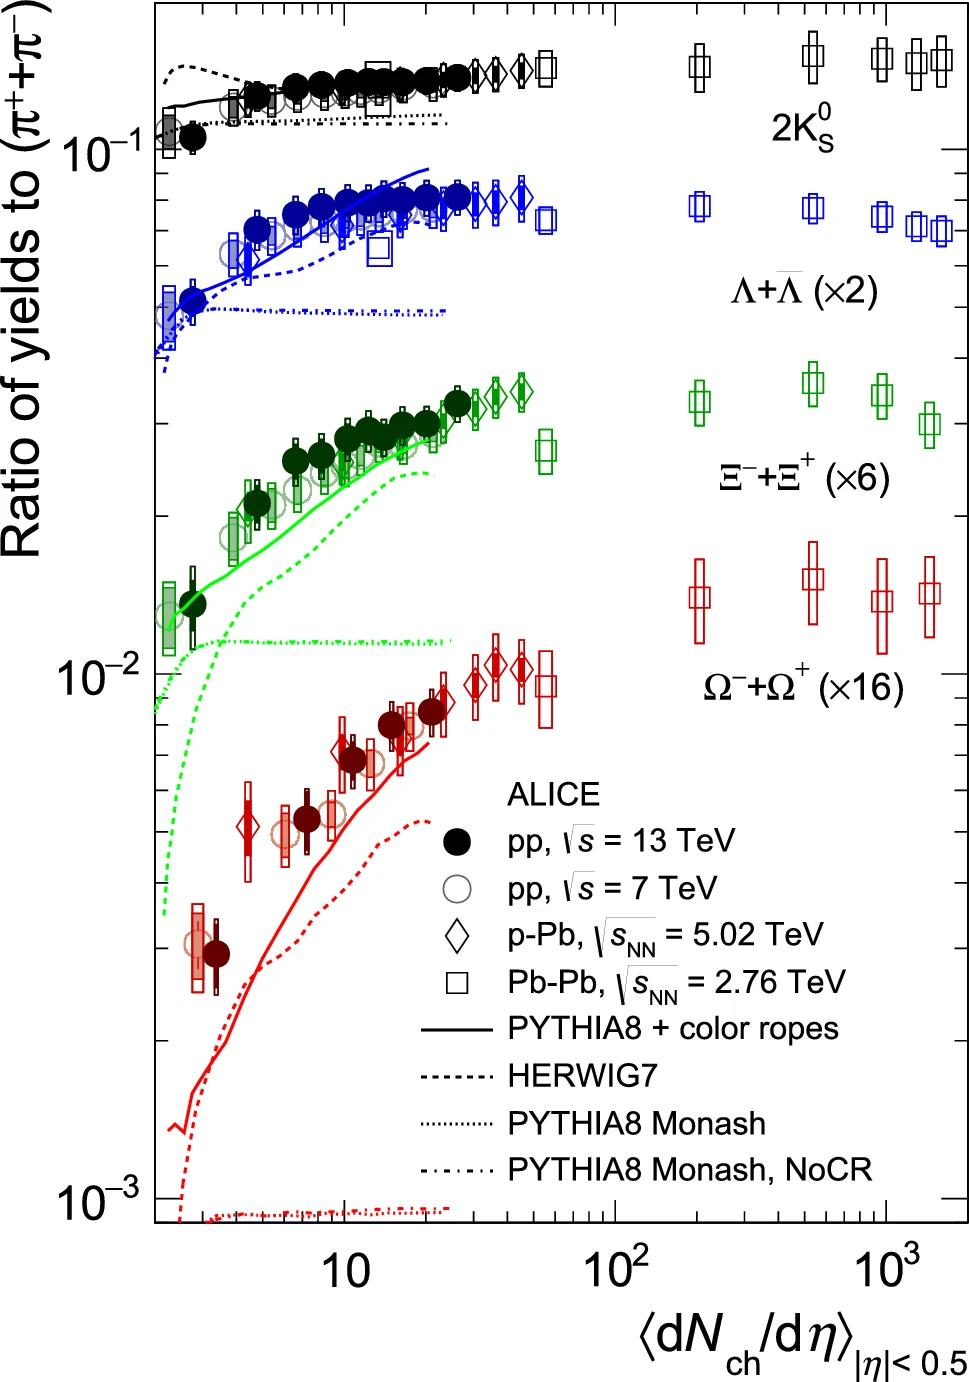
\includegraphics[width=0.55\textwidth, valign=t]{Figs/Chapter6/img.jpg}
	\label{fig:PythiaVsStrangenessEnhancement}
} 
\subfigure[]{
	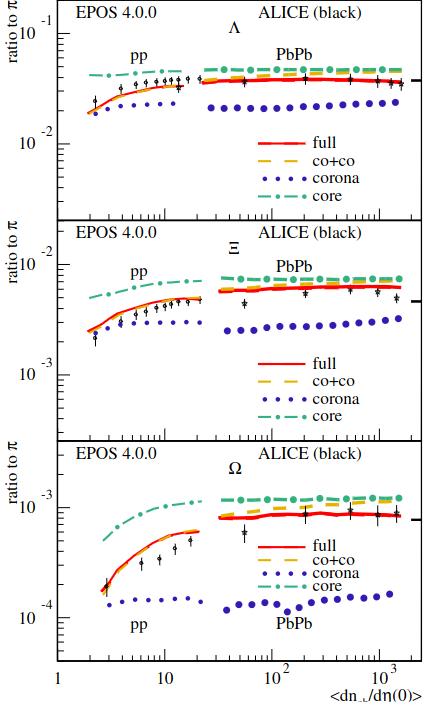
\includegraphics[width=0.6\textwidth, valign=t]{Figs/Chapter6/StrangenessEnhancement_CoreCorona.png}
	\label{fig:EposVsStrangenessEnhancement}
} 
\caption{Integrated strange hadrons-to-pions yield ratio as a function of the average charged particle multiplicity at mid-rapidity in ALICE, compared to different MC predictions. On the left, it is measured in pp at \sqrtS = 7 and 13 \tev, p-Pb at \sqrtSnn = 5.02 \tev, Pb-Pb collisions at \sqrtSnn = 2.76 \tev , and compared to \Pythiaeight and \Herwig\cite{acharyaMultiplicityDependencePi2020}; on the right, these are measurements in pp at \sqrtS = 7 \tev and Pb-Pb collisions at \sqrtSnn~=~2.76~\tev, with different predictions from \Epos \cite{wernerCorecoronaProcedureMicrocanonical2023}.}
	\label{fig:MCModelStrangenessEnhancement}
\end{figure}

One of the key historical signatures of QGP is the strangeness enhancement which consists in the enhanced yield of multi-strange hadrons in heavy ion collisions with respect to small systems (\Sec\ref{subsec:StrangenessEnhanement}). Such yields also scale smoothly with the charged particle multiplicity in pp collisions (\Sec\ref{subsec:ComparisonPP}, \fig\ref{fig:StrangenessEnhancement}). Different models using fundamentally different mechanisms manage to reproduce qualitatively this trend (\fig\ref{fig:MCModelStrangenessEnhancement}). On one hand, \Pythia \cite{bierlichComprehensiveGuidePhysics2022}\cite{skandsTuningPYTHIAMonash2014} models the quark hadronisation using the Lund Strings; these correspond to gluon fields, that break whenever the string tension energy is high enough and thus leading to the formation of hadrons, similarly as in \fig\ref{fig:QuarkFragmentation}. Both pp and heavy-ion collision physics originate from the interaction of these strings, \ie this approach assumes the absence of a QGP. On the other hand, \Epos \cite{wernerCorecoronaProcedureMicrocanonical2023} relies natively on multiple parton scatterings, further organised with a core-corona distinction in the collision: a dense core hosting a QGP-like collective medium, surrounded by a hadron gas corona \cite{wernerAnalysingRadialFlow2014}. So far, neither of these approaches has been able to provide an unambiguous explanation on the emergence of collective phenomena in small systems. Further experimental inputs are required in order to distinguish them, and finally identify the hadron production mechanisms. 

A way to shed more light on the situation is to perform more multi-differential study, typically of the angular and rapidity correlations between different hadron species. These bring informations on the quark production, and consequently on the hadronisation. Two hadrons produced out of the breaking of a colour string into a quark-antiquark pair, as modeled by \Pythia, should exhibit a strong local correlation. On the other hand, if the quarks are produced in the early stage of the collision -- the so-called \say{prehadrons} in \Epos framework \cite{wernerCorecoronaProcedureMicrocanonical2023} -- and hadronise later, that correlation should vanish.

\begin{figure}[t]
\centering
%\hspace*{-1.25cm}
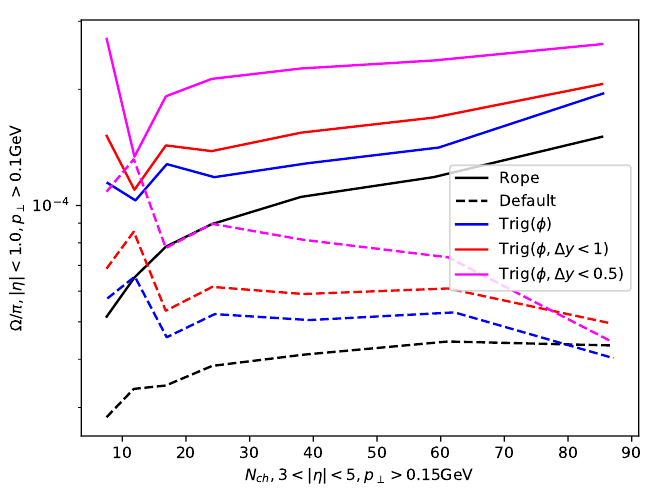
\includegraphics[width=0.8\textwidth]{Figs/Chapter6/PredictionPythia_Bierlich.png}
\caption{\Pythiaeight predictions for the \rmOmega-to-\rmPiPM yield ratio as a function of the charged particle multiplicity in pp collisions at \sqrtS =  13 \tev, in presence of a \rmPhiMes resonance (colour lines) or not (black line). The default \Pythia configuration (\Pythiaeight, tune: Monash 2013) is indicated in dashed line, whereas the full curves represent the case with the colour ropes enabled.}
	\label{fig:PredictionPythia_Bierlich}
\end{figure}

One example of such measurement comes from the \Pythia experts; since strangeness is conserved by the strong interaction, the number of strange hadrons is expected to be exactly compensated by the number of anti-strange hadrons, leading to a correlation between these hadrons\footnote{As a side note, since all the strange hadrons are correlated, one can control to some extent the strangeness content within an event using a trigger on strange particle, \rmXi or \rmOmega for example.}. In particular, within the standard Lund string framework, multi-strange baryons can be produced through a diquark-antidiaquark string breaking. However, the \say{recent} developments towards heavy-ion collisions -- namely the colour reconnection and colour rope \cite{christiansenStringFormationLeading2015}\cite{bierlichEffectsOverlappingStrings2015a}\cite{adolfssonQCDChallengesPp2020} -- offer new production mechanisms. As a consequence, it is predicted that i) the \rmOmega abundancy increases in presence of a \rmPhiMes in the event, and ii) this enhancement gets more prominent as the gap in rapidity between these two particles decreases \fig\ref{fig:PredictionPythia_Bierlich}.

So far, no such correlation has ever been measured. A similar observable has been studied recently \cite{adolfssonStudyXiHadron2020}, that analyses the angular correlations between the multi-strange baryon \rmXiPM and \pOrPbar, \rmPiPM, \rmKPM, \rmLambdaPM, \rmXiPM itself. It was not extended to \rmPhiMes resonance nor repeated with \rmOmega baryons, though. Therefore, this analysis aims to check this prediction via the measurement of correlated production of \rmOmega and \rmPhiMes over all the pp collisions at a centre-of-mass energy of 13 \tev collected throughout the LHC Run-2 by ALICE. In order to reduce as much as possible the background contamination, such measurement requires a trigger with a high purity, and thus good control capabilities over the amount of signal and the background for the trigger. For that reason and contrarily to the \Pythia's prediction, the trigger is on the \rmOmega particles and not the \rmPhiMes, the former offering a more governable purity.

Since the \rmXi baryon is much more produced than the \rmOmega, two measurements are performed : first, the correlated production of \rmXi and \rmPhiMes, and then the one of \rmOmega and \rmPhiMes. In this way, the feasibility of such measurement can be checked on the \rmXi, and if so, it will be repeated with the \rmOmega.\\

By design, this kind of analysis relies on two categories of particles: the \textit{trigger particles}, which is then correlated to the particles of interest in the event, the \textit{associated particles}. In the present chapter, the term \textit{trigger particle} designates either a \rmXi or a \rmOmega baryon, and the \textit{associated particle} corresponds to the \rmPhiMes resonance.


\section{Data samples and event selection}

\subsection{The data samples}

Considering their relatively low yield -- about $ 2 \times 10^{-2}$ \rmXi and $\sim 1.85 \times 10^{-3}$ \rmOmega, and $\sim 3.8 \times 10^{-2}$ \rmPhiMes at mid-rapidity \cite{alicecollaborationProductionLightflavorHadrons2020} -- the correlation between these particles requires all the data available. Therefore, this second analysis employs the same real and simulated data samples as in the first one, in \chap\ref{chap:CPTAnalysis}. It means that all pp collisions at centre-of-mass energy of 13 \tev collected in 2016, 2017 and 2018 are put to use (\Sec\ref{subsec:DataSamples}). 

Contrarily to the first analysis, this one exploits data in AOD format, as it does not necessitate such a fine control over the data reconstruction. The analysed events also come from the second reconstruction cycle, the pass-2.

\subsection{The event selection}

All the event selections employed in the first analysis (\Sec\ref{subsec:EventSelection}) are also applied here. These are complemented by an additional requirement on the type of event.

The behaviour of the hadronic interactions at high energies is typically described by the Regge theory\cite{collinsIntroductionReggeTheory1977}. There exists two classes of interaction: the elastic collisions -- when the initial and final states of the interaction are the same -- and inelastic (\INEL) collisions, that involve the production of new particles. The latter subdivides into two categories: the diffractive and non-diffractive processes. The former combines single and double diffractive processes. Within the framework of the Regge theory, the diffractive processes occur respectively when either or both incoming protons become an excited system -- due to the exchange of Pomerons --, that later decay into stable final-state particles emitted close to the mother direction, \ie close to beam, at very forward rapidity \cite{alicecollaborationMeasurementInelasticSingle2013}.

This analysis focuses on hadrons produced in inelastic collisions at mid-rapidity, hence originating \textit{a priori} from non-diffractive processes. Experimentally, this kind of inelastic collisions are selected by requiring, at least, one reconstructed SPD tracklet in $\abspseudorap < 1 $. This condition is commonly refered as \INELZero\footnote{Note that \INELZero events do not correspond to the total number of inelastic collisions \INEL, due to the acceptance and efficiency of the \INELZero condition, the beam-induced background selections, the number of un-reconstructed events (because no preliminary primary vertex could be formed for example, \Sec\ref{subsubsec:PreliminaryVertex}). In fact, for MB$_{\rm AND}$, the \INELZero encompasses about 76.3$_{-0.8}^{+2.2}$\% of the total number of inelastic collisions \cite{alicecollaborationALICEDataPreparation2023}.}.\\

\begin{table}[t]
    \centering
    \begin{tabular}{c|ccccc}
    \noalign{\smallskip}\hline \noalign{\smallskip}
    Multiplicity Class & \upperRomannumeral{1} & \upperRomannumeral{2} & \upperRomannumeral{3} & \upperRomannumeral{4} & \upperRomannumeral{5} \\
	\sigmaIdx[]/\sigmaIdx[\INELZero] & 0-0.01\% & 0.01-0.1\% & 0.1-0.5\% & 0.5-1\% & 1-5\% \\	        
	$\langle \dNchdeta \rangle$ & $35.37_{-0.86}^{+0.92}$ & $30.89_{-0.51}^{+0.57}$ & $26.96_{-0.30}^{+0.37}$ & $24.23_{-0.30}^{+0.36}$ & $20.02_{-0.22}^{+0.27}$ \\
	\noalign{\smallskip}\hline \noalign{\smallskip}
	Multiplicity Class & \upperRomannumeral{6} & \upperRomannumeral{7} & \upperRomannumeral{8} & \upperRomannumeral{9} & \upperRomannumeral{10} \\
	\sigmaIdx[]/\sigmaIdx[\INELZero] & 5-10\% & 10-15\% & 15-20\% & 20-30\% & 30-40\% \\
	$\langle \dNchdeta \rangle$ & $16.17_{-0.18}^{+0.22}$ & $13.77_{-0.16}^{+0.19}$ & $12.04_{-0.14}^{+0.17}$ & $10.02_{-0.11}^{+0.14}$ & $7.95_{-0.09}^{+0.11}$ \\
	\noalign{\smallskip}\hline \noalign{\smallskip}
	Multiplicity Class & \upperRomannumeral{11} & \upperRomannumeral{12} & \upperRomannumeral{13} & & \\
	\sigmaIdx[]/\sigmaIdx[\INELZero] & 40-50\% & 50-70\% & 70-100\% & & \\
	$\langle \dNchdeta \rangle$ & $6.32_{-0.07}^{+0.09}$ & $4.50_{-0.05}^{+0.07}$ & $2.55_{-0.03}^{+0.04}$ &  &  \\
    \noalign{\smallskip}\hline \noalign{\smallskip}
    \end{tabular}
    \caption{Event multiplicity classes, with the corresponding fraction of the total inelastic cross section \INELZero (\sigmaIdx[]/\sigmaIdx[\INELZero]) and average charged particle multiplicity at mid-rapidity, $\langle \dNchdeta \rangle$. Table taken from \cite{alicecollaborationEnhancedProductionMultistrange2017}\cite{alicecollaborationPseudorapidityTransversemomentumDistributions2016}.}
    \label{tab:MultiplicityClasses}
\end{table}

Moreover, two estimators can be considered for the multiplicity determination: the total charge deposited in the VZERO scintillator arrays in $-3.7 < \eta < -1.7$ and $2.8 < \eta < 5.1$ (VZERO-M amplitude, \Sec\ref{subsubsec:EventMultDependence}); the number of reconstructed SPD tracklets in $\abspseudorap < 1$ ($\rmNTracklet^{\abspseudorap < 1}$). Although the choice between these two estimators seems innocent/arbitrary, notice that they cover different pseudo-rapidity regions: the former estimates the multiplicity (at mid-rapidity) based on the energy deposited at forward rapidity, while the latter counts the number of tracklets at mid-rapidity. This difference may have some implications. Since the observable is a yield ratio at mid-rapidity, the considered particle and/or its decay products may contribute to the number of reconstructed SPD tracklets, thus self-biasing the multiplicity event. In general, the separation between the region of interest and the volume covered by the multiplicity estimator should be as large as possible, in order to avoid or limit this auto-correlation. For that reason, the VZERO-M is taken as default multiplicity estimator. 

It follows that the events are divided into thirteen multiplicity classes, presented in \tab\ref{tab:MultiplicityClasses}. The \Sec\ref{sec:CascadeResonanceCorrelationAnalysis} will show that the reconstruction of cascade and a \rmPhiMes resonance in the same event requires at least five tracks. Therefore, the correlations between these two hadrons are measured for events comprised between the 50\% with the lowest multiplicity to the 1\% with the highest multiplicity, 


\section{Analysis of the multi-strange baryon-\rmPhiMes correlation}
\label{sec:CascadeResonanceCorrelationAnalysis}

\subsection{The correlation function}

The objective is to measure the correlation between a multi-strange baryon, either \rmXiPM or \rmOmegaPM, and a \rmPhiMes meson. Their correlation is evaluated by associating them in pairs, and observing how the pair population is distributed according to a given variable. More precisely, the focus here is on the correlated yield of \rmPhiMes meson in events containing, at least, one multi-strange baryon. Therefore, the observable should be the per-trigger yield of the \rmPhiMes meson as a function of the difference in rapidity, azimuthal angle between the trigger particle and the associated particles, and the multiplicity of the event, 

\begin{equation}
\frac{1}{N_{\text{trigger}}} \cdot \dNXdX{pairs}{$y$} = \frac{1}{\dNXdy{cascade}} \cdot \dNXdX{pairs}{$y$} \left(\Delta \varphi, \Delta y, \text{multiplicity} \right),
\label{eq:IdealCorrelationFunction}
\end{equation}
where the $N_{\text{pairs}}$ corresponds to the number of cascade-\rmPhiMes pairs.\\

It will become clear in the next sections that a multi-differential observable such as in \eq\ref{eq:IdealCorrelationFunction} cannot be measured currently with the LHC Run-2 data, due to the lack of statistics. Nonetheless, this correlation may still be investigated, although less differentially. Along this line, this analysis proposes to measure the per-trigger yield as a function of one variable at a time, \ie
\begin{align}
&\frac{1}{\dNXdy{cascade}} \cdot \dNXdXdy{pairs}{$\Delta y$},\\
&\frac{1}{\dNXdy{cascade}} \cdot \dNXdXdy{pairs}{$\Delta \varphi$}.
\end{align}\\

A few words on the analysis strategy before proceeding. Therefore, only events containing a \rmXi or \rmOmega candidate are selected; from these, the particles of interest are reconstructed using the selections in \Sec\ref{subsec:ResonanceSelections}. After calculating the invariant mass of each candidate, they are sorted as a function of their \pT\footnote{This is necessary in order to correct for the detector acceptance and the reconstruction efficiency (\Sec\ref{subsec:AccEff}).} and -- only for the particles of interest -- the difference of rapidity $\Delta y$ and azimuthal angle $\Delta \varphi$ with respect to the trigger particle. The yields of both species are extracted from their respective invariant mass distributions, for each \pT, $\Delta y$, and $\Delta \varphi $ bins, as presented in \Sec\ref{subsec:CascadeResonanceSignalExtraction}. 

In the present measurement, the associated particles comprise solely the \rmPhiMes. However, the analysis has been designed in view of extending the correlations to other kind of hadrons, namely \pOrPbar, \rmPiPM, \rmKPM, \rmKstarZero, \rmKzeroS, \rmLambdaPM, \rmXiPM and \rmOmegaPM.

\begin{table}[h]
    \centering
    \begin{tabular}{>{\centering\arraybackslash}b{1.5cm}@{\hspace{0.3cm}} >{\centering\arraybackslash}b{1.75cm}@{\hspace{0.3cm}} >{\centering\arraybackslash}b{2.85cm}@{\hspace{0.3cm}} >{\centering\arraybackslash}b{3.6cm}@{\hspace{0.3cm}} >{\centering\arraybackslash}b{2.5cm}@{\hspace{0.3cm}} >{\centering\arraybackslash}b{1cm}@{\hspace{0.3cm}}}
    \noalign{\smallskip}\hline\noalign{\smallskip}
	Particle & Quark content & Mass (\mmass) & Lifetime \cTau (cm) or Width $\Gamma$ (\mmass) & Dominant decay channel & B.R.\\	
    \noalign{\smallskip}\hline \noalign{\smallskip}
    	
	\rmPhiMes & $s \bar{s}$ & $1019.461 \pm 0.020$ & $\Gamma = 4.249$ & \rmKplus \rmKminus & 49.1\%\\
	
    \noalign{\smallskip}\hline \noalign{\smallskip}
    
    \rmLambda (\rmAlambda) & $u d s$ ($\bar{u}\bar{d}\bar{s}$) & $1115.683 \pm 0.006$ &  $\cTau = 7.89$ & \proton \piMinus (\pbar \piPlus) & 63.9\% \\
    
    \noalign{\smallskip}\hline \noalign{\smallskip}    
    
    \rmXiM (\rmAxiP) & $dss$ ($\bar{d}\bar{s}\bar{s}$) & $1321.71 \pm 0.07$ & $\cTau = 4.91$ & \rmLambda \piMinus (\rmAlambda \piPlus) & 99.9\% \\	
    \noalign{\smallskip}\hline \noalign{\smallskip}
    
	\rmOmegaM (\rmAomegaP) & $sss$ ($\bar{s}\bar{s}\bar{s}$) & $1672.45 \pm 0.23$ & $\cTau = 2.461$ & \rmLambda \rmKminus (\rmAlambda \rmKplus) & 67.8\%\\    
    \noalign{\smallskip}\hline\noalign{\smallskip}
    \end{tabular}
    \caption{A few characteristics, as of 2023, of the \rmLambda, \rmXi, \rmOmega hyperons and the \rmPhiMes meson resonance: quark content, mass, relative mass difference values with their associated uncertainties and their dominant decay channel as well as the corresponding branching ratio \cite{particledatagroupReviewParticlePhysics2022}.}\label{tab:ResonanceV0CascPDGMass}
\end{table}

The multi-strange baryons being already introduced in details in \chap\ref{chap:V0CascReconstruction} and \chap\ref{chap:CPTAnalysis}, we will be concentrating on the \rmPhiMes resonance. As presented in \tab\ref{tab:ResonanceV0CascPDGMass}, it has a mass of 1019.461 \mev and a width of 4.249 \mev, equivalent to a lifetime of approximately 46 \fm. It mainly decays via strong interaction into a pair of oppositely charged kaons with a branching ratio of 49.1\%, $\rmPhiMes \rightarrow \rmKplus \rmKminus$, as depicted in \fig\ref{fig:ResonanceDecay}. In the following, the \rmPhiMes will be studied in this decay channel.

The \rmPhiMes resonance is reconstructed by forming pairs of oppositely charged tracks;  similarly to the V0s, the positively charged daughter is called the \textit{positive} particle, the other the \textit{negative} particle. As a consequence of the strong nature of the decay, its short flight distance makes the decay vertex undistinguable from the primary interaction point. Thereby, the misassociated pairs cannot be discarded using geometrical selections -- as opposed to the topological reconstruction of V0s and cascades --, leading to a substantial combinatorial background. This is the reason why it was decided to consider the multi-strange baryons as trigger particles, instead of the \rmPhiMes meson. This background can be evaluated and subtracted by making use of two techniques, presented later in \Sec\ref{subsec:ResonanceSelections}. \\

\begin{SCfigure}[][h]
\centering
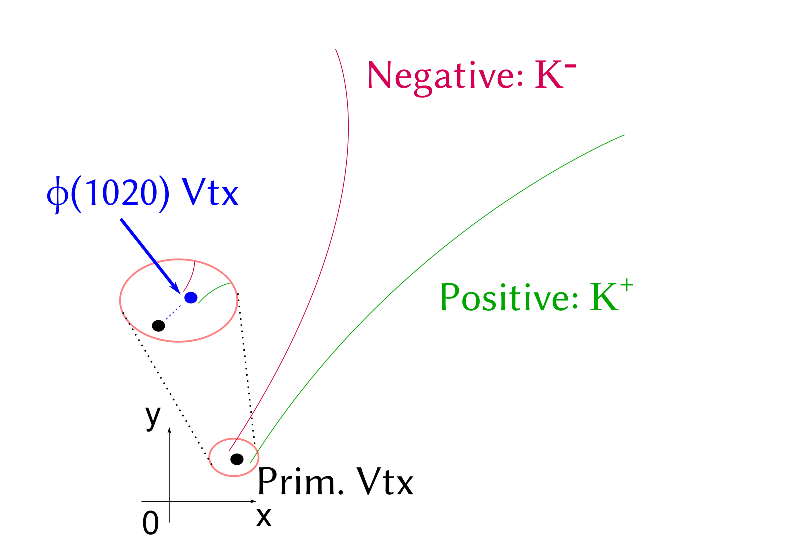
\includegraphics[width=0.65\textwidth]{Figs/Chapter6/Schema-PhiDecay.eps}
\caption{Scheme of the resonance decay of the \rmPhiMes meson. Modified version of the original figure \cite{maireFourTypesCascade2011}.}
	\label{fig:ResonanceDecay}
\end{SCfigure}


\subsection{Cascade candidate selections}

As in \chap\ref{chap:CPTAnalysis}, the identification of multi-strange baryons relies on their characteristic cascade decay channel. Their reconstruction therefore exploits the same topological and kinematic selection variables, \Sec\ref{subsec:TrackSelections} and \ref{subsec:V0CascSelections}. These are presented in \tab\ref{tab:TriggerParticleSelections}.

There is however one important difference with respect to the first analysis. While the latter measures the mass integrated over all the \pT bins\footnote{There is one exception in \Sec\ref{subsubsec:MassDependenceOnPt}, where the \pT-differential measurement of the mass is performed in order to check the stability of the results with the transverse momentum.}, the objective here is to extract the yield of both trigger and associated particles, these being obtained from their \pT-differential production rate. 

\begin{equation}
\dNdy = \int_{0}^{+\infty} \dNdptdy \text{d}\pT
\end{equation}

\begin{table}[t]
    \centering
    \begin{tabular}{c|c|c}
    \noalign{\smallskip}\hline \noalign{\smallskip}
    \bf Candidate variable & Selections \rmXiPM & Selections \rmOmegaPM \\
    \noalign{\smallskip}\hline \noalign{\smallskip}    
    Cascade \pT interval (\gmom) & \multicolumn{2}{c}{$0.6 < \pT < 6.5$} \\
    Cascade rapidity interval & \multicolumn{2}{c}{\absrap < 0.5} \\
    Competing mass rejection (\gmass) & - & > 0.008 \\
    MC association (MC only) & \multicolumn{2}{c}{Correct identity assumption} \\ 

    \noalign{\smallskip}\hline \noalign{\smallskip}
    \bf Track variable & Selections \rmXiPM & Selections \rmOmegaPM \\
    \noalign{\smallskip}\hline \noalign{\smallskip}
    Pseudo-rapidity interval & \multicolumn{2}{c}{\abspseudorap < 0.8} \\
    TPC refit & \multicolumn{2}{c}{\CheckGr} \\
    Nbr of crossed TPC readout rows & \multicolumn{2}{c}{ > 70} \\
    $\Nsigma^{\rm TPC}$ & \multicolumn{2}{c}{< 3} \\
    \multirow{ 2}{*}{Out-of-bunch pile-up rejection} & \multicolumn{2}{c}{at least one track with} \\
     & \multicolumn{2}{c}{ITS-TOF matching} \\
    
    \noalign{\smallskip}\hline \noalign{\smallskip}
    \bf Topological variable & Selections \rmXiPM & Selections \rmOmegaPM \\
    \noalign{\smallskip}\hline \noalign{\smallskip}
    
    \multicolumn{3}{l}{\textbf{V0}} \\
    V0 decay radius (\cm) & > 1.2 & > 1.1\\
    V0 cosine of pointing angle & \multicolumn{2}{c}{> 0.97}\\
    |$m$($V0$) - \mPDG\rmLambda| (\gmass) & \multicolumn{2}{c}{< 0.008} \\
    DCA proton to prim. vtx (\cm) & \multicolumn{2}{c}{> 0.03} \\
    DCA pion to prim. vtx (\cm) & \multicolumn{2}{c}{> 0.04} \\
    DCA V0 to prim. vtx (\cm) & \multicolumn{2}{c}{> 0.06} \\
    DCA between V0 daughters (std dev) & \multicolumn{2}{c}{< 1.5} \\
    \noalign{\smallskip}\hline \noalign{\smallskip}
    
    \multicolumn{3}{l}{\textbf{Cascade}} \\
    Cascade decay radius (\cm) & > 0.6 & > 0.5 \\
    Cascade Lifetime (\cm) & \multicolumn{2}{c}{< 3 $\times$ \cTau}\\
    DCA bachelor to prim. vtx (\cm) & \multicolumn{2}{c}{> 0.04} \\
    DCA between cascade daughters (std dev) & \multicolumn{2}{c}{< 1.3} \\
    Cascade cosine of pointing angle & \multicolumn{2}{c}{> 0.998} \\
    Bachelor-proton pointing angle (rad) & \multicolumn{2}{c}{> 0.04} \\
    
    \noalign{\smallskip}\hline \noalign{\smallskip}
    \end{tabular}
    \caption{Summary of the topological and track selections, as well as the associated cut values, used in the reconstruction of \rmXiPM and \rmOmegaPM in pp events at \sqrtS = 13 \tev. The \textit{competing mass rejection} refers to the removal of the background contamination from other mass hypotheses (\Sec\ref{subsubsec:InvariantMassSelection})}\label{tab:TriggerParticleSelections}
\end{table}

Thereby, the candidates are sorted as a function of their transverse momentum according to, for \rmXiPM baryons, thirteen \pT intervals: 
\begin{quote}
$\left[ 0.6 ; 1.0 \right) \gmom$,  $\left[ 1.0 ; 1.2 \right) \gmom$, $\left[ 1.2; 1.4 \right)\gmom$, $\left[1.4 ; 1.6 \right) \gmom$, $\left[ 1.6 ; 1.8 \right) \gmom$, 
$\left[ 1.8 ; 2.0 \right) \gmom$, $\left[ 2.0 ; 2.2 \right) \gmom$, $\left[ 2.2 ; 2.5 \right) \gmom$, $\left[ 2.5 ; 2.9 \right) \gmom$,  $\left[ 2.9 ;  3.4 \right) \gmom$,
$\left[ 3.4 ; 4.0 \right) \gmom$, $\left[ 4.0 ; 5.0 \right) \gmom$, $\left[ 5.0 ; 6.5 \right)\gmom$. 
\end{quote}

For what concerns the measurement of the \rmOmegaPM hyperons, due to their lower statistics, six intervals are being used:
\begin{quote}
$\left[ 1.0 ; 1.6 \right) \gmom$,  $\left[ 1.6 ; 2.2 \right) \gmom$, $\left[ 2.2; 2.6 \right)\gmom$, $\left[2.6 ; 3.0 \right) \gmom$, $\left[ 3.0 ; 3.8 \right) \gmom$, $\left[ 3.8 ; 6.5 \right) \gmom$.
\end{quote}

\subsection{Resonance candidate selections}
\label{subsec:ResonanceSelections}

As explained in the header of this section, the \rmPhiMes meson candidates are reconstructed as a pair of \rmKplus and \rmKminus. Since the decay topology cannot be exploited to reduce the amount of combinatorial background, most of the selection criteria focus on the quality of daughter tracks\footnote{In this analysis, the focus is on the \rmPhiMes yield in presence of a multi-strange baryon. However, note that the same considerations would also apply in the case of the \rmKstarZero resonance, that decays strongly into a \rmKPM and a \rmPiPM at $\sim$100\%.}. These can be found in \tab\ref{tab:PhiSel}.

\begin{table}[h]
    \centering
    \begin{tabular}{c|c}
    \noalign{\smallskip} \hline \noalign{\smallskip}
    \bf Candidate variable & Selection criterion \\
    \noalign{\smallskip} \hline \noalign{\smallskip}    
    Resonance rapidity interval & \absrap < 0.5 \\
    MC association (MC only) & Correct identity assumption \\ 
    \noalign{\smallskip} \hline \noalign{\smallskip}
    \bf Track variable & Selection criterion \\
    \noalign{\smallskip} \hline \noalign{\smallskip}
    \pT interval (\gmom) & 0.15 < \pT < 20 \\
    Pseudo-rapidity interval & \abspseudorap < 0.8 \\
    ITS refit & \CheckGr \\
    TPC refit & \CheckGr \\
    Kink Topology & - \\
    $\Nsigma^{\rm TPC}$  & < 3 \\    
    $\Nsigma^{\rm TOF}$  (if available) & < 3 \\    
    Nbr of crossed TPC readout rows & > 70 \\
	Fraction of crossed TPC readout & \multirow{2}*{$\geq$ 0.8} \\
	rows over findable clusters & \\
	Goodness of the TPC standalone track, $\chi_\textsc{TPC}^2 / N_{\rm cluster}$ & < 4 \\
	Global and TPC standalone track matching, $\chi_\textsc{TPC-CG}^2$ & < 36 \\
	Goodness of the ITS standalone track, $\chi_\textsc{ITS}^2 / N_{\rm cluster}$ & < 36 \\
	Nbr of associated SPD clusters & $\geq$ 1 \\
	DCA to prim. vtx (cm) & < 0.0105 + 0.035 \pT$^{-1.01}$ \\
	DCA to prim. vtx along z (cm) & < 2 \\
    \noalign{\smallskip} \hline \noalign{\smallskip}
    \end{tabular}
    \caption{Summary of the track and candidate selections used for the reconstruction of \rmPhiMes.}\label{tab:PhiSel}
\end{table}

Beyond the track selections in common with the hyperons (\Sec\ref{subsec:TrackSelections}), only tracks of sufficiently good quality are selected by requiring a reduced $\chi^2$ up to 36 and 4, for the ITS- and TPC-standalone tracks respectively\footnote{The tighter selection on the goodness of the TPC standalone track is related to the fact that TPC is the main tracking device in ALICE and so, contributes the most to the track quality.}. The agreement between the TPC-standalone track, constrained to the preliminary primary vertex (\Sec\ref{subsec:EventReco}), and global track is quantified by the so-called \textit{golden} $\chi^{2}$; its value should be smaller than 36. Along the same line, each track must have passed the final refit in the ITS, and be associated with at least one hit in the innermost ITS layers, the most granular detector of the experiment. To ensure a good momentum resolution, the fraction of found crossed TPC readout rows over the number of findable clusters must reach at least 80\%.  

Since the decay point cannot be resolved from the primary vertex, the formation of a resonance candidate uses primary tracks, contrarily to the V0 and cascade reconstructions. These are identified by imposing that their distance of closest approach to the primary vertex is smaller than a critical value. In particular, in the transverse plane, the latter is given by a \pT-dependent \textit{ad-hoc} formula in order to be even more selective.

Further combinatorial background is suppressed by applying PID criteria. It is required that each track agrees with a \rmKPM mass hypothesis within $n_{\sigma}^{\rm TPC} = \pm 3$. Whenever it matches a hit in the TOF detector\footnote{Since a substantial amount of particles do not reach or cannot be matched with a hit in the TOF detector, the associated hadron identification capabilities can only be used whenever they are available, in complement to other PID informations; otherwise, this would drastically affect the track reconstruction efficiency.}, the time-of-flight informations supplement the selection on the nature of the decay daughter using the PID estimator in \eq\ref{eq:PIDestimatorTOF}, $n_{\sigma}^{\rm TOF}$.\\


Finally, any pair of tracks satisfying the above criteria and lying at mid-rapidity,  \absrap < 0.5, is considered as a \rmPhiMes meson candidate. Their measurement is performed in the following eight \pT intervals:
\begin{quote}
$\left[0.4; 0.8\right) \gmom$, $\left[0.8; 1.2\right) \gmom$, $\left[1.2; 1.8\right) \gmom$, $\left[1.8; 2.6\right) \gmom$, $\left[2.6; 3.4\right) \gmom$, $\left[3.4; 4.2\right)\gmom$, $\left[4.2; 5\right)\gmom$, $\left[5; 11\right) \gmom$.
\end{quote}


\subsection{The raw signal extraction}
\label{subsec:CascadeResonanceSignalExtraction}

\subsubsection{In the case of multi-strange baryons}

The raw signal extraction for the trigger particle follows the very same procedure as in the first analysis. Therefore, the invariant mass peak is modelled by a triple Gaussian (\eq\ref{eq:Gaus}), and the background by a an exponential function. The amount of raw signal and background are estimated by bin counting, over the same regions as in \Sec\ref{subsec:MassExtraction}. 

The \figs\ref{fig:InvMassXiMinusVPt}, \ref{fig:InvMassXiPlusVPt}, \ref{fig:InvMassOmegaMinusVsPt}, \ref{fig:InvMassOmegaPlusVsPt} show the invariant mass distribution in the different \pT intervals for \rmXiM, \rmAxiP, \rmOmegaM and \rmAomegaP respectively.

\begin{landscape}
\begin{figure}[h]
	\centering
	\includegraphics[width=1.45\textwidth]{Figs/Chapter6/InvMassXiMinus\_Correlated.eps}
\caption{Invariant mass spectra of the \rmXiM candidates in pp collisions at \sqrtS = 13 \tev, fitted by the combination of three Gaussian functions for the peak and a decreasing exponential function for the background. The amounts of signal and background have been obtained via bin counting in the peak (red area) and side-bands region (gray area).}
	\label{fig:InvMassXiMinusVPt}
\end{figure}

\begin{figure}[h]
	\centering
	\includegraphics[width=1.45\textwidth]{Figs/Chapter6/InvMassXiPlus\_Correlated.eps}
\caption{Invariant mass spectra of the \rmAxiP candidates in pp collisions at \sqrtS = 13 \tev, fitted by the combination of three Gaussian functions for the peak and a decreasing exponential function for the background. The amounts of signal and background have been obtained via bin counting in the peak (red area) and side-bands region (gray area).}
	\label{fig:InvMassXiPlusVPt}
\end{figure}

\end{landscape}

\begin{figure}[!p]
	\hspace*{-1.5cm}
	\includegraphics[width=1.25\textwidth]{Figs/Chapter6/InvMassOmegaMinus\_Correlated.eps}
\caption{Invariant mass spectra of the \rmOmegaM candidates in pp collisions at \sqrtS = 13 \tev, fitted by the combination of three Gaussian functions for the peak and a decreasing exponential function for the background. The amounts of signal and background have been obtained via bin counting in the peak (red area) and side-bands region (gray area).}
	\label{fig:InvMassOmegaMinusVsPt}
\end{figure}

\begin{figure}[!p]
	\hspace*{-1.5cm}
	\includegraphics[width=1.25\textwidth]{Figs/Chapter6/InvMassOmegaPlus\_Correlated.eps}
\caption{Invariant mass spectra of the \rmAomegaP candidates in pp collisions at \sqrtS = 13 \tev, fitted by the combination of three Gaussian functions for the peak and a decreasing exponential function for the background. The amounts of signal and background have been obtained via bin counting in the peak (red area) and side-bands region (gray area).}
	\label{fig:InvMassOmegaPlusVsPt}
\end{figure}

\clearpage
%\begin{table}[h]
%    \centering
%    \begin{tabular}{b{2cm}@{\hspace{1cm}} b{2.5cm}@{\hspace{0.5cm}} b{2cm}@{\hspace{0.5cm}} b{3cm}@{\hspace{0.5cm}} b{2cm}@{\hspace{0.1cm}}}
%    \noalign{\smallskip}\hline\noalign{\smallskip}
%	 & \multicolumn{4}{c}{\rmXiM (\rmAxiP)} \\	
%	\pT (\gmom) & Reduced $\chi^2$ & Raw signal & Background & Purity \\	
%    \noalign{\smallskip}\hline \noalign{\smallskip}
%    $\left[ 0.6 ; 1.0 \right)$ & 12.689 & 11.273 & 5.051 & 4.707\\
%    	$\left[ 1.0 ; 1.2 \right)$ &  1 237 666 & 1 168 882 & 65 232 & 63 842\\
%    	$\left[ 1.2; 1.4 \right)$ & 55 375 & 51 269 & 5758 & 5490 \\
%    	$\left[1.4 ; 1.6 \right)$ & 22.4 & 22.8 & 11.4 & 11.7 \\
%    	$\left[ 1.6 ; 1.8 \right)$ & 95.7\% & 95.8\% & 91.8\% & 92.1\% \\
%    $\left[ 1.8 ; 2.2 \right)$ & 1089 & 1059 & 245 & 243 \\
%    $\left[ 2.2 ; 2.5 \right)$ & 1089 & 1059 & 245 & 243 \\
%    $\left[ 2.5 ; 2.9 \right)$ & 1089 & 1059 & 245 & 243 \\
%    $\left[ 2.9 ; 3.4 \right)$ & 1089 & 1059 & 245 & 243 \\
%    $\left[ 3.4 ; 4.0 \right)$ & 1089 & 1059 & 245 & 243 \\
%    $\left[ 4.0 ; 5.0 \right)$ & 1089 & 1059 & 245 & 243 \\
%    $\left[ 5.0 ; 6.5 \right)$ & 1089 & 1059 & 245 & 243 \\
%    \noalign{\smallskip}\hline\noalign{\smallskip}
%    \end{tabular}
%    \caption{Results from the fit of the invariant mass distributions in \fig\ref{fig:InvMassCascades} concerning the samples of \rmXiM, \rmAxiP, \rmOmegaM and \rmAomegaP. Therefore, this table reports the reduced $\chi^{2}$, raw signal, background, ratio $S/B$, purity and signal significance.}\label{tab:FitQuantities}
%\end{table}

\subsubsection{In the case of \rmPhiMes meson}
\label{subsubsec:RawSignalExtractionPhiMes}

The invariant mass of each resonance candidate is calculated using the \eq\ref{eq:ResonanceInvMass} and making the assumption of a \rmKPM mass for both decay daughters. The top left figure in \fig\ref{fig:InvMassPhiResVsPt} presents the invariant mass spectrum of the \rmPhiMes meson candidates with a transverse momentum between 400 and 800 \mmom. 
\begin{align}
M_{\rm candidate}^2 \left[ \rmPhiMes \right] &= ( E_{\rm pos.} + E_{\rm neg.} )^2 - ( \vec{p}_{\rm pos.} + \vec{p}_{\rm neg.})^2 \\
&= \Big(\sqrt{ \vec{p}_{\rm pos.}^2 + m_{\rm pos.}^2} + \sqrt{ \vec{p}_{\rm neg.}^2 + m_{\rm neg.}^2}\Big)^2 - ( \vec{p}_{\rm pos.} + \vec{p}_{\rm neg.})^2\\
&= \Big(\sqrt{ \vec{p}_{\rm pos.}^2 + m_{\rm K^{+}}^2} + \sqrt{ \vec{p}_{\rm neg.}^2 + m_{\rm K^{-}}^2}\Big)^2 - ( \vec{p}_{\rm pos.} + \vec{p}_{\rm neg.})^2 \label{eq:ResonanceInvMass}
\end{align}
An excess of counts emerges around the tabulated mass of the \rmPhiMes, $\mPDG = 1019.461$ \mmass, on top of a smooth background. The latter dominates the invariant mass distribution, and derives \textit{a priori} mainly from combinatorics of the tracks. The origin of the background being known, it can thus be removed\footnote{Alternatively, one could try to find a functional form that describes correctly the shape of the background, as it was done in \chap\ref{chap:CPTAnalysis}. For instance, here, it could be modeled by a second order polynomial.}. The basic idea consists to reproduce the background shape by forming uncorrelated pairs of tracks. There exist two approaches\footnote{In fact, there also exist a third approach. These resonances are formed out of two oppositely charged, \ie unlike-charge, tracks. Particles of the same charge are uncorrelated with respect to the \rmPhiMes decay. Hence, by pairing like-charge tracks, \rmKplus\rmKplus and \rmKminus\rmKminus, the combinatorial background can be estimated. However, this procedure has been implemented in the analysis, and so will not be used.}:
\begin{itemize}
\item[$\bullet$] \textbf{Event mixing technique:} by definition, particles originating from different events could not have been produced together, and so are uncorrelated. Consequently, the association of tracks from different events should \textit{in principle} result in combinatorial background. This is the core concept of event mixing.
Therefore, each positively charged track passing the above selections (\Sec\ref{subsec:ResonanceSelections}) gets paired to a negatively charged track from another event, under the exact same set of cuts, and vice versa. Each event is mixed with five other events at most.
In order to estimate correctly the combinatorial background, the mixing has to be performed between events with similar collision kinematics. To ensure that, it is required that i) the longitudinal position of their primary vertex agrees within a range of $\pm$ 1 \cm, and ii) their difference in terms of event multiplicity should be sufficiently low, such that they belong to the same multiplicity class. Moreover, since the several events are involved in the mixing, the mixed-event invariant mass distribution needs to be normalised, such that it fits the same-event distribution in certain invariant mass region. This normalisation is usually performed far from the peak, in the side-bands regions purely populated by combinatorial background.
\item[$\bullet$] \textbf{Rotating procedure:} the excess of counts in the invariant mass distributions originates from correlated pairs of \rmKplus and \rmKminus due to the \rmPhiMes meson decay. If the correlation of the pair could somehow be broken, the invariant mass spectrum should be populated solely by combinatorial background. This can be achieved by considering the already formed pairs of kaons from the same event and rotating one of track by a significant amount, typically by an angle of 180\textdegree. 
\end{itemize}

\begin{figure}[t]
	\hspace{-2.cm}
%	\centering
	\includegraphics[width=1.35\textwidth, angle=0]{Figs/Chapter6/InvMassResonance\_Correlated.eps}
\caption{Top left panel: Unlike-charge and mixed-event invariant mass distribution for \pT between 0.4 and 0.8 \gmom. The other panels: Invariant mass spectra of the \rmPhiMes meson candidates in pp collisions at \sqrtS = 13 \tev, fitted by the sum of a Voigt function for the peak and a linear function for the residual background. The amounts of signal have been obtained as explained in \Sec\ref{subsubsec:RawSignalExtractionPhiMes}, while the background has been obtained via bin counting in the region covered by the red area, that is 1.005 and 1.035 \gmass.}
	\label{fig:InvMassPhiResVsPt}
\end{figure}

The event mixing technique is taken as the default option, as it will later facilitate another part of the analysis \Sec\ref{subsec:EvtMixingCascPhi}. The rotating procedure is going to be used in the systematic study. 

Whatever the considered approach, the combinatorial background is subtracted from the invariant distribution, yielding to the other panels in \figs\ref{fig:InvMassPhiResVsPt}. The invariant mass now sits on top of a small residual background. The signal is separated from the background through a (log-)likelyhood method. 

The ideal signal for a resonance should exhibit a Breit-Wigner shape \cite{breitCaptureSlowNeutrons1936}. However, the invariant mass peak rather corresponds to the convolution of Breit-Wigner and Gaussian -- due to the smearing induced by the detectors response -- distributions, meaning a Voigt profile (\eq\ref{eq:Voigt}). 

\begin{equation}
\dNdX{\mInv} = A \cdot \frac{\Gamma}{(2\pi)^{3/2} \sigma} \int\limits_{-\infty}^{\infty} \text{exp} \left[ -\frac{(\mInv - m')^2}{2\sigma^2} \right] \frac{1}{(m' - \mu)^2 + \Gamma^2/4} \text{d} m',
\end{equation}\label{eq:Voigt}
where:
\begin{itemize}
\item[$\bullet$] $A$ coincides with the integral of the function from $0$ to $+\infty$,
\item[$\bullet$] $\mu$ corresponds to the centre of the Voigt function,
\item[$\bullet$] $\Gamma$ is the resonance width,
\item[$\bullet$] and $\sigma$ describes the width of the Gaussian.
\end{itemize}

Only this function is considered for the peak description. Here, two types of Voigtian fits are considered: one with the resonance width fixed at the nominal value ($\Gamma = 4.249$ \mmass), the other where it is allowed to vary freely. Concerning the residual background, as in the first analysis, different shapes can be considered: constant, linear, exponential functions, second order polynomial. However, the linear function will be taken as our default option.\\

If the fitting procedure converges, the signal and background are estimated. Since the Voigt function does not decrease as fast as a Gaussian with the distance to the centre, the amount of raw signal and background have to be evaluated differently. As a consequence, the peak region for \rmPhiMes resonance is defined in fixed invariant mass range, $\left[1.005 ; 1.035\right] \gmass$, which contains most of the signal and some background. The raw signal is obtained by counting the number of candidates in this region and subtracting the background population; the latter is given by the integral of the background function over the same region, hence $S_{\rm counting} = \left(S+B\right)_{\rm counting} - B_{\rm integral}$. The rest of the signal population sits outside the peak region, from 0.987354\footnote{This value corresponds to $2 m_{\rm K^{\pm}} = 0.987354 \gmass$ with $m_{\rm K^{\pm}} = 0.493677 \gmass$ \cite{particledatagroupReviewParticlePhysics2022}. The population of \rmPhiMes cannot be found below this mass value because it is kinematically forbidden.} to $1.005$ \gmass and $1.035$ to $+\infty$ \gmass. Consequently, the integral of the Voigt function in these two regions provides an estimation of the missing signal population, which is then incorporated in the total raw signal $S = S_{\rm counting}\left( 1.005 ; 1.035 \right) + S_{\rm integral}\left( 0.987354 ; 1.005\right) + S_{\rm integral} \left( 1.035 ; +\infty\right)$\footnote{In the analysis, the peak function is not integrated to $+$ infinity, but rather up to a large mass value with respect to the \rmPhiMes mass -- that is 5 \gmass -- such that most of the missing raw signal has been taken into account.}.

\subsection{Fraction of background cascade}
\label{subsec:FractionOfBkgCascade}

As explained in the header of this section, the correlation between cascade and resonances goes through pairs of particle candidates. Thereby, as illustrated in \tab\ref{tab:CorrelationTab}, there exist four types of pairs depending on whether they are signal or background candidates.

\begin{table}[h]
\centering
\begin{tabular}{ | c | c | c | }
	\hline
	\backslashbox{\rmXiPM or \rmOmegaPM}{\rmPhiMes}
    & Signal candidate & Background candidate \\
	\hline
    Signal candidate & Signal-Signal & Signal-Background \\
    Background candidate & \cellcolor{red!50} Background-Signal & \cellcolor{red!50}Background-Background \\
	\hline
\end{tabular}
\caption{Four types of cascade-resonance correlation in the analysis, depending on the cascade and resonance candidates. The red cells represent the correlations with a background trigger candidate, that must be removed.}
\label{tab:CorrelationTab}
\end{table}


In the ideal case, only correlation between a true \rmXiPM or \rmOmegaPM and an actual \rmPhiMes should be observed. As explained in \Sec\ref{subsec:ResonanceSelections}, the contribution from the background resonances is already removed bin-by-bin first using an event mixing technique, and then the raw signal of \rmPhiMes is isolated from the residual background through a fit with a linear function. The only remaining source of correlation with background candidate comes from the multi-strange baryons. Considering the purity of the sample, the contribution of the cascade background candidates could be assumed as negligible. This means that
\begin{equation}
\begin{split}
\frac{1}{N_{\text{trigger}}} \cdot \dNXdXdy{pairs}{$X$} &= \left.\frac{1}{N_{\text{trigger}}(S)} \cdot \dNXdXdy{\rmPhiMes}{$X$}\right|_{(S)\ \textrm{trigger} -\  (S)\ \textrm{associated pairs}}\\
&\simeq \left.\frac{1}{N_{\text{trigger}}(S+B)} \cdot \dNXdXdy{pairs}{$X$}\right|_{(S+B)\ \textrm{trigger} -\  (S)\ \textrm{associated pairs}},
\end{split}
\end{equation}
where $X$ corresponds to either $\Delta y$ or $\Delta \varphi$, $(S+B)$ signifies signal and background candidates, and $(S)$ is for pure signal candidates.\\

An attempt is made to get as precise as possible. To that end, two measurements are performed: one in which cascades in the peak region are correlated to resonance candidates, and another with cascades from the side-bands region instead. Each of them provides a set of invariant mass distributions for the associated particles as a function of their rapidity and/or azimuthal angle gap with respect to the trigger particle. 

%\begin{equation}
%\begin{array}{lcl}
%	\frac{1}{N_{\text{trigger}}} \cdot \dNXdXdy{\rmPhiMes}{$X$}&=& \left.\frac{1}{N_{\text{trigger}}(S)} \cdot \dNXdXdy{\rmPhiMes}{$X$}\right|_{(S)\ \textrm{trigger} -\  (S)\ \textrm{associated pairs}}\\
%  & & \\
%  &=& \frac{1}{N_{\text{trigger}}(S+B) - N_{\text{trigger}}(B)} \cdot \\
%  & & \\
%  & &\qquad \Big[ \left.\dNXdXdy{\rmPhiMes}{$X$}\right|_{(S+B)\ \textrm{trigger}  -\ (S)\ \textrm{associated pairs}} \\
%  & & \\
%  & &\qquad \qquad- \left.\dNXdXdy{\rmPhiMes}{$X$}\right|_{(B)\ \textrm{trigger}  -\ (S)\ \textrm{associated pairs}} \Big].
%\end{array}
%\end{equation}

\begin{equation}
\begin{split}
\frac{1}{N_{\text{trigger}}} \cdot \dNXdXdy{\rmPhiMes}{$X$} &= \left.\frac{1}{N_{\text{trigger}}(S)} \cdot \dNXdXdy{\rmPhiMes}{$X$}\right|_{(S)\ \textrm{trigger} -\  (S)\ \textrm{associated pairs}}\\
&= \frac{1}{N_{\text{trigger}}(S+B) - N_{\text{trigger}}(B)} \cdot\\ 
&\hspace{1cm} \Bigg[ \left.\dNXdXdy{\rmPhiMes}{$y$}\right|_{(S+B)\ \textrm{trigger} -\ (S)\ \textrm{associated pairs}} \\
&\hspace{2cm} - \left.\dNXdX{\rmPhiMes}{$y$}\right|_{(B)\ \textrm{trigger}  -\ (S)\ \textrm{associated pairs}} \Bigg].
\end{split}
\end{equation}

\subsection{Acceptance and efficiency corrections}
\label{subsec:AccEff}

The raw signal quantifies the amount of multi-strange baryons or \rmPhiMes resonances reconstructed within the acceptance of the ALICE detector, and satisfying the selections in \tabs\ref{tab:TriggerParticleSelections} and \ref{tab:PhiSel}. In fact, this quantity corresponds to a fraction of the total number of particles produced in the fiducial volume $\absrap < 0.5$ due to i) the limited acceptance of the detector that prevents the reconstruction of tracks within certain region of the ALICE apparatus (beyond $\abspseudorap < 0.8$, deadzones), and ii) the finite reconstruction and selection efficiencies of the cascade and resonance decays. This fraction can be estimated using MC simulations.

In principle, the correction on the raw signal breaks down into two terms, one for each of the aforementioned contributions: the \textit{acceptance}, that corresponds to the fraction of reconstructable particles in the fiducial volume among the total number of generated particles within the desired rapidity region ($\absrap < 0.5$), and the \textit{efficiency} -- or \textit{reconstruction efficiency} -- given by the ratio of the number of reconstructed hadrons over the number of reconstructable ones in the same rapidity interval. The product of these two terms provides the acceptance and efficiency correction factors (\eq\ref{eq:AccEff}).

\begin{align}
\textrm{Acceptance} \times \textrm{Efficiency} &= \frac{N_{\rm generated\ in\ |y| < y_{\rm fid.}}^{\rm daughter\ in\ acc.}}{N_{\rm generated\ in\ |y| < 0.5}} \times \frac{N_{\rm reconstructed\ in\ |y| < y_{\rm fid.}}}{N_{\rm generated\ in\ |y| < y_{\rm fid.}}^{\rm daughter\ in\ acc.}}\label{eq:AccEff}\\
&= \frac{N_{\rm reconstructed\ in\ |y| < y_{\rm fid.}}}{N_{\rm generated\ in\ |y| < 0.5}}\label{eq:FinalAccEff}
\end{align}

For the sake of simplicity, instead of evaluating these correction factors individually, this analysis goes directly for the product of the two (\eq\ref{eq:FinalAccEff}). Since the above selections impact differently low-\pT and high-\pT candidates, these acceptance and efficiency correction factors do depend strongly on the transverse momentum. Therefore, they have to be determined for every \pT interval. \\

%Moreover, note that the branching ratio of the considered particle stands as an upper bound for the reconstruction efficiency, and so for the acceptance $\times$ efficiency.\\

\begin{figure}[t]
\begin{minipage}[c]{0.4\linewidth}
\begin{align*}
\left[\begin{array}{>{\centering\arraybackslash}b{4.5cm}@{\hspace{0.2cm}}|>{\centering\arraybackslash}b{1.1cm}@{}}
      \cellcolor{green!50} & \cellcolor{red!50}\\
      \cellcolor{green!50} & \cellcolor{red!50}\textsc{\footnotesize T}\\
      \cellcolor{green!50} \textsc{\footnotesize T \& C} & \cellcolor{red!50}\textsc{\footnotesize \&}  \\  
      \cellcolor{green!50} & \cellcolor{red!50}\textsc{\footnotesize \cancel{C}} \\
      \cellcolor{green!50} & \cellcolor{red!50}\\    \hline
      \textsc{\footnotesize \cancel{T} \& C} &  \textsc{\footnotesize \cancel{T} \& \cancel{C}}
    \end{array}\right] \\
\end{align*}
\end{minipage}\hfill
\begin{minipage}[c]{0.4\linewidth}
\begin{align*}
\left[\begin{array}{>{\centering\arraybackslash}b{1.1cm}@{\hspace{0.2cm}}|>{\centering\arraybackslash}b{4.5cm}@{}}
      \cellcolor{green!50} \textsc{\footnotesize T \& C} & \cellcolor{red!50} \textsc{\footnotesize T \& \cancel{C}}  \\ \hline  
       &  \\
      \textsc{\footnotesize \cancel{T}} &  \\
      \textsc{\footnotesize \&} &  \textsc{\footnotesize \cancel{T} \& \cancel{C}}\\
      \textsc{\footnotesize C} &  \\
       &  
    \end{array}\right] \\
\end{align*}
\end{minipage}
\caption{Study of the correlated yield between the trigger and associated particles in two different cases. The area occupied by each cell provides its relative contribution to the correlated production. Four contributions are considered: a trigger particle has been found/detected/reconstructed in the event (\textsc{T}) and it is correlated to at least one associated particle (\textsc{C}); there is no correlation between these particles (\textsc{T \& \cancel{C}}); a trigger particle is present and correlated to an associated particle, though it is not reconstructed (\textsc{\cancel{T} \& C}); the trigger particle is not found and is not correlated to the particle of interest (\textsc{\cancel{T} \& \cancel{C}}). The green area corresponds to the measurement at stake, while the red zone represents the contribution accounted for in \Sec\ref{subsec:EvtMixingCascPhi}. The un-coloured areas are not seen in the present analysis.}
\label{fig:TriggeredContribution}
\end{figure}

These corrections aim to compensate for the un-detected and/or\break un-reconstructed particles in the analysis. Hence, most measurements apply such corrections on both trigger and associated particles. While this makes sense in the latter case, it is more dubious for the former ones: by correcting the cascade raw signal, one increases basically the number of such hadrons in the analysis. Those being used as a trigger, this is equivalent to increase the number of triggered events. Depending on whether those additional/corrected events contains a \rmPhiMes meson or not, whether they are reconstructed or not, whether they are correlated to the trigger particle or not, this will most certainly affect the estimation of the \rmXiPM-\rmPhiMes and \rmOmegaPM-\rmPhiMes correlations. If, as depicted in the left panel of \fig\ref{fig:TriggeredContribution}, such correlation in non-triggered event turns out to be small, the previous concerns may reasonably be neglected in first approximation. Conversely, in the configuration shown in the right panel of \fig\ref{fig:TriggeredContribution}, one should be extremely cautious on how to correct the trigger particle yield.

Due to the non-trivial application of the acceptance $\times$ efficiency correction factors on the \emph{trigger} particle, the present measurement restricts only to correlations in triggered events\footnote{The same argument can be made concerning an eventual extrapolation of the particle yield to low transverse momentum, which is also done in most measurements of this nature. Considering our minimum \pT threshold -- 0.4 for the \rmPhiMes, 0.6 \gmom for the \rmXiPM, 1 \gmom for the \rmOmegaPM --, an extrapolation down to $\pT = 0$ would imply an increase of the \rmPhiMes, \rmXiPM, \rmOmegaPM yields by about 15-20\%, 35\% and 45\% respectively. The impact of such extrapolation is thus non-negligible. Nevertheless, this will not be done in the present analysis for the same reason as the trigger particles are corrected for the limited acceptance and reconstruction efficiency of the detector.}. This means that the acceptance and efficiency corrections concern solely the associated particles, namely the \rmPhiMes. The \fig\ref{fig:EfficiencyRsn} shows their acceptance and reconstruction efficiencies for the \pT intervals defined in \Sec\ref{subsec:ResonanceSelections}.

\begin{figure}[h]
%	\hspace{-2.cm}
	\centering
	\includegraphics[width=1.\textwidth, angle=0]{Figs/Chapter6/Efficiency\_Resonance.eps}
\caption{Acceptance and reconstruction efficiency (acceptance $\times$ efficiency $\times$ B.R.) of the \rmPhiMes resonance at mid-rapidity ($\absrap < 0.5$) using the set of selections in \tab\ref{tab:PhiSel}.}
	\label{fig:EfficiencyRsn}
\end{figure}

\subsection{Accounting for the uncorrelated cascade-resonance pairs}
\label{subsec:EvtMixingCascPhi}

As for the \rmPhiMes meson reconstruction, there is no way to tell \textit{a priori} which cascade is correlated to a resonance, and vice versa. All the possible combinations have to be exhausted. This inevitably leads to the formation of uncorrelated cascade-\rmPhiMes pairs. 

Such contribution can be removed using the exact same methods as those used for subtracting the combinatorial background of resonances: either via an event mixing technique or rotating procedure (\Sec\ref{subsec:ResonanceSelections}). Our choice went on the first option, purely for simplicity. On the practical side, by re-using the same mixed-event list as for the \rmPhiMes, the longest part of procedure is already done, making the implementation of the event mixing technique straighforward.

The whole analysis chain needs to be repeated, including the previous elements \Sec\ref{subsec:FractionOfBkgCascade} and \ref{subsec:AccEff}, but this time, only trigger-associated pairs originating from different event (given by the event mixing) are considered. A new per-trigger yield ratio is then extracted, 
\begin{equation}
\frac{1}{N_{\text{trigger}}} \cdot \dNXdXdyMix{pairs}{$X$}.
\end{equation}

To account for the uncorrelated pairs of particles, the correlation function has to be re-defined such that it is given by the ratio of the measured per-trigger yield to the one obtained in different event. In other words, this means that the final correlation function corresponds in fact to 
\begin{equation}
\frac{1}{N_{\text{trigger}}} \cdot \dNXdXdy{pairs}{$X$} \Bigg/ \frac{1}{A} \cdot \frac{1}{N_{\text{trigger}}} \cdot \dNXdXdyMix{pairs}{$X$}.
\end{equation}
Here $A$ is a normalisation factor that controls the contribution of the uncorrelated pairs in the final result. It plays a critical role as, depending on its estimation, the value of the final correlation function can change drastically and so the physical interpretation. To avoid that, one has to identify an \say{anchor point} in the same-event distribution where no correlations are expected. Based on that, the normalisation can be determined by considering that the correlated and uncorrelated distributions should coincide at that precise point of the phase space. This is totally analogue to what was done in the \rmPhiMes reconstruction, when subtracting the combinatorial background; in that case, the \say{anchor} corresponded to a certain range in the invariant mass distribution\footnote{Ideally, we should also consider a range of points for the determination of the normalisation factor. However, due to the limited of statistics, the distributions are populated by only a few number of points, making it impossible.}.

\subsection{Preliminary results}
\label{subsec:PreliminaryResultsCorrelation}

\begin{figure}[t]
%	\hspace{-2.cm}
\centering
\subfigure[]
	{
	\includegraphics[width=0.8\textwidth, angle=0]{Figs/Chapter6/PerTriggerYield\_VsRap\_XiPhi.eps}
	\label{fig:PerTriggerYieldXiRap}
	}
\centering
\subfigure[]
	{
	\includegraphics[width=0.8\textwidth, angle=0]{Figs/Chapter6/PerTriggerYield\_VsPhi\_XiPhi.eps}
	\label{fig:PerTriggerYieldXiPhi}
	}
\caption{Measured \rmPhiMes resonance yield per \rmXiPM trigger as a function of (a) the rapidity gap, $\Delta y$, and (b) the difference in azimuth, $\Delta \varphi$, at mid-rapidity ($\absrap < 0.5$) in minimum-bias pp collisions at a centre-of-mass energy of 13 \tev. The blue points represent the same event distribution, while the green ones show the contribution from uncorrelated trigger-associated particle pairs. The error bars represent only the statistical uncertainty. These two distributions have been obtained using the default set of selections, in \tabs\ref{tab:TriggerParticleSelections} and \ref{tab:PhiSel}.}
	\label{fig:PerTriggerYieldXi}
\end{figure}

The \figs\ref{fig:PerTriggerYieldXi} show the measured \rmPhiMes resonance yield per \rmXiPM trigger as a function of the difference in rapidity $\Delta y$ and in azimuth $\Delta \varphi$, in the same event in blue, and from different event in green. Here, the mixed-event distributions have been normalised to the point with the largest rapidity gap on the negative side\footnote{One could also have considered the point with the largest rapidity gap on the positive side; both choice are \textit{a priori} equivalent. An alternative could be to take the average of the two most extreme $\Delta y$ values.}, and the bin corresponding to an angular separation of $\pi/2$. One can reasonably assume that there should no correlation in those bins, or if there is any, it should be mild. The mixed-event distribution forms some kind of pedestal, with a tent-like shape\footnote{As the correlation in $(\Delta y, \Delta \varphi)$ can not be studied due to the limited statistics, one has to resort on imagination. The front view of the tent is the green distribution in the \fig\ref{fig:PerTriggerYieldXiRap}, while the side view corresponds to the mixed-event distribution in \fig\ref{fig:PerTriggerYieldXiPhi}.}, characteristic of the contribution from uncorrelated particle pairs such as cascades originating from the underlying event or mini-jets.



\begin{figure}[t]
%	\hspace{-2.cm}
\centering
\subfigure[]
	{
	\includegraphics[width=0.8\textwidth, angle=0]{Figs/Chapter6/PerTriggerYield\_VsRap\_XiPhi\_Ratio.eps}
	\label{fig:PerTriggerYieldXiRapRatio}
	}
\centering
\subfigure[]
	{
	\includegraphics[width=0.8\textwidth, angle=0]{Figs/Chapter6/PerTriggerYield\_VsPhi\_XiPhi\_Ratio.eps}
	\label{fig:PerTriggerYieldXiPhiRatio}
	}
\caption{Correlations between the \rmXiPM hyperons and \rmPhiMes resonances, at mid-rapidity ($\absrap < 0.5$), as a function of (a) their difference in rapidity, $\Delta y$, and (b) in azimuth, $\Delta \varphi$, in minimum-bias pp collisions at a centre-of-mass energy of 13 \tev. The error bars represent only the statistical uncertainty. This distribution has been obtained using the default set of selections, in \tabs\ref{tab:TriggerParticleSelections} and \ref{tab:PhiSel}.}
	\label{fig:PerTriggerYieldXiRatio}
\end{figure}


The ratio of the same event and mixed-event distributions provides the final correlation function, as explained in \Sec\ref{subsec:EvtMixingCascPhi}. It can be found in \figs\ref{fig:PerTriggerYieldXiRatio}. The number of trigger-associated particle pairs increases in the \fig\ref{fig:PerTriggerYieldXiRapRatio}, going from the far negative $\Delta y$ side to the far positive side. Considering the statistical uncertainty, no conclusion can be drawn at the moment concerning an enhancement of the \rmPhiMes production when close in rapidity to a \rmXiPM baryon ($\Delta y \sim 0$).

However, on \fig\ref{fig:PerTriggerYieldXiPhiRatio}, the \rmPhiMes resonance yield increases by approximately 35\% when the latter lies in the vicinity, in azimuth, of a double strange baryon ($\Delta \varphi \sim 0$). One would also expect a peak on the away-side of the trigger particle, \ie $\Delta \varphi = \pi$. These are typically \rmPhiMes emitted in the opposite direction of the \rmXiPM. However, with the present statistical uncertainties, no such peak is observed.\\

The initial goal being to correlate a \rmOmegaPM baryon to \rmPhiMes meson, an attempt has been made to obtain similar results but with \rmOmegaPM as trigger particle. However, it turns out that the available statistics in minimum-bias pp collisions is not enough to perform differential analysis. Combining all the LHC Run-2 data, the number of \rmPhiMes resonances in the same event as a \rmOmegaPM amounts to 7 191. To perform the same study as for the \rmXi baryons, the analysis should move towards high-multiplicity pp collisions, where the statistics is much higher.

For the time being, the analysis will continue on minimum-bias pp collisions, but focusing only on events containing a \rmXiPM hyperon. The \fig\ref{fig:PerTriggerYieldXiPhiRatio} suggests an angular correlation between the \rmPhiMes and \rmXiPM, as the resonances appear 35\% more abundant when produced close in azimuth to a trigger particle. However, before drawing any conclusion, one should first study and estimate the systematic uncertainties associated to our measurement.

\section{Study of the systematic uncertainties}

\subsection{Topological and track selections}
\label{subsec:SystTopoTrackSelCorrelation}

A possible source of systematic bias may arise from the identification of the cascade and resonance candidates. To evaluate it, the different set of selections should be varied and the effect on the \textit{corrected} results, assessed. 

This could be achieved following the same approach as the one exposed in \Sec\ref{subsubsec:SystTopoMass}, that is via the random generation of several thousands of sets of selections. However, the limited statistics prevent such a granular study. Instead, a more standard approach is used. Different class of selections shall be defined and used to perform a new measurement. The deviation of the results with respect to the standard/default configuration provides an estimate of the systematic uncertainty due to the choice of candidate selections.

It should be mentioned that only the \say{statistically significant} variations are considered. What establishes a deviation as such is given by Roger Barlow \cite{barlowSLUOLecturesStatistics2000}\cite{barlowSystematicErrorsFacts2002}, and is already exposed in the header of \Sec\ref{sec:SystStudy}. In the first analysis, the threshold for a statistically significant variation has been set at $\sigmaBarlow\simeq 1$. The critical aspect of the first analysis being on the precise study of the systematic biases, it made sense to resort to a low threshold. Since the key word for the present analysis not \say{precision} -- as in \chap\ref{chap:CPTAnalysis} --  but \say{efficiency}, the threshold has been elevated to $\sigmaBarlow\simeq 2$.\\

This study is performed for both the multi-strange baryons and \rmPhiMes resonances, although separately.

\subsubsection{Multi-strange baryon identification}

Different set of cuts have been defined: \say{very loose}, \say{loose}, \say{tight} and \say{very tight}. Behind these labels, there is a signal variation between five to ten percent, in order to be \say{harsh} enough to cause an observable effect without losing all the signal but not too \say{gentle} to induce no change in the results. The precise value of each cuts have been inspired on the study performed in the first analysis, as well as in \cite{alicecollaborationMultiplicityDependenceMulti2020}. These are detailed in the \tab\ref{tab:SystTopoCorrelatedAnalysisXi}. The variations induced by each class of cuts on the correlation function are displayed in \figs\ref{fig:SystPerTriggerYieldXiRatioCascade}. 

\begin{table}[t]
	\hspace{-1.5cm}
    \begin{tabular}{c|c|c|c|c|c}
    \noalign{\smallskip}\hline \noalign{\smallskip}
    \bf Track variable & Very loose & Loose & Default & Tight & Very tight \\
    \noalign{\smallskip}\hline \noalign{\smallskip}
    Nbr of crossed TPC readout rows &  & & > 70 & > 80 & > 90\\
    $\Nsigma^{\rm TPC}$ & < 5 & < 4 & < 3 & < 2.5 & < 2\\
    
    \noalign{\smallskip}\hline \noalign{\smallskip}
    \bf Topological variable \\
    \noalign{\smallskip}\hline \noalign{\smallskip}
    
    \multicolumn{3}{l}{\textbf{V0}} \\
    V0 decay radius (\cm) & > 1 & > 1.1 & > 1.2 & > 3 & > 5\\
    V0 cosine of pointing angle & & & > 0.97 & > 0.98 & > 0.99\\
    |$m$($V0$) - \mPDG\rmLambda| (\gmass) & < 0.010 & < 0.009 & < 0.008 & < 0.007 & < 0.006\\
    DCA proton to prim. vtx (\cm) & & & > 0.03 & > 0.07 & > 0.1 \\
    DCA pion to prim. vtx (\cm) &  & > 0.03 & > 0.04 & > 0.15 & > 0.3 \\
    DCA V0 to prim. vtx (\cm) & & & > 0.06 & > 0.1 & > 0.13 \\
    DCA between V0 daughters (std dev) & < 2 & < 1.8  & < 1.5 & < 1.2 & < 1.0 \\
    \noalign{\smallskip}\hline \noalign{\smallskip}
    
    \multicolumn{3}{l}{\textbf{Cascade}} \\
    Cascade decay radius (\cm) & > 0.4 & > 0.5 & > 0.6 & > 0.8 & > 1 \\
    Cascade Lifetime (\cm) & < 5 \cTau & < 4 \cTau & < 3 \cTau & < 2.5 \cTau &\\
    DCA bachelor to prim. vtx (\cm) &  & > 0.03 & > 0.04 & > 0.1 & > 0.17\\
    DCA between cascade daughters (std dev) & < 2 & < 1.6 & < 1.3 & < 1.0 & < 0.8 \\
    Cascade cosine of pointing angle & > 0.99 & > 0.995 & > 0.998 & > 0.9985 & > 0.999 \\
    Bachelor-proton pointing angle (rad) & > 0.02 & > 0.03 & > 0.04 & > 0.045 & > 0.05 \\
    
    \noalign{\smallskip}\hline \noalign{\smallskip}
    \end{tabular}
    \caption{Summary of the five configurations -- the default as well as four variants -- on the topological and track selections employed in the identification the \rmXiPM in pp events at \sqrtS = 13 \tev. When a value is missing, the preceding selection is considered. These sets of selections have been determined based on the signal variation study carried out in the first analysis (\Sec\ref{subsec:SystTopoAndTrackSelections}), in conjunction with the ones used in \cite{alicecollaborationMultiplicityDependenceMulti2020}.}\label{tab:SystTopoCorrelatedAnalysisXi}
\end{table}

%\begin{table}[t]
%	\hspace{-1.2cm}
%    \begin{tabular}{c|c|c|c|c|c}
%    \noalign{\smallskip}\hline \noalign{\smallskip}
%    \bf Candidate variable & Very loose & Loose & Default & Tight & Very tight \\
%    \noalign{\smallskip}\hline \noalign{\smallskip}
%    Competing mass rejection (\gmass) & > 0.006 & > 0.007 & > 0.008 & > 0.009 & > 0.010\\
%    \noalign{\smallskip}\hline \noalign{\smallskip}
%    \bf Track variable \\
%    \noalign{\smallskip}\hline \noalign{\smallskip}
%    Nbr of crossed TPC readout rows &  & & > 70 & > 80 & > 90\\
%    $\Nsigma^{\rm TPC}$ & < 5 & < 4 & < 3 & < 2.5 & < 2\\
%    
%    \noalign{\smallskip}\hline \noalign{\smallskip}
%    \bf Topological variable \\
%    \noalign{\smallskip}\hline \noalign{\smallskip}
%    
%    \multicolumn{3}{l}{\textbf{V0}} \\
%    V0 decay radius (\cm) & & > 1.0 & > 1.1 & > 2.5 & > 3.5\\
%    V0 cosine of pointing angle &  &  & > 0.97 & > 0.98 & > 0.99\\
%    |$m$($V0$) - \mPDG\rmLambda| (\gmass) & < 0.010 & < 0.009 & < 0.008 & < 0.007 & < 0.006\\
%    DCA proton to prim. vtx (\cm) &  &  & > 0.03 & > 0.07 & > 0.1 \\
%    DCA pion to prim. vtx (\cm) &  & > 0.03 & > 0.04 & > 0.15 & > 0.3 \\
%    DCA V0 to prim. vtx (\cm) & & & > 0.06 & > 0.08 & > 0.1 \\
%    DCA between V0 daughters (std dev) & < 2 & < 1.8  & < 1.5 & < 1.2 & < 1.0 \\
%    \noalign{\smallskip}\hline \noalign{\smallskip}
%    
%    \multicolumn{3}{l}{\textbf{Cascade}} \\
%    Cascade decay radius (\cm) & > 0.3 & > 0.4 & > 0.5 & > 0.6 & > 0.8 \\
%    Cascade Lifetime (\cm) & < 5 \cTau & < 4 \cTau & < 3 \cTau & < 2.5 \cTau &\\
%    DCA bachelor to prim. vtx (\cm) &  & > 0.03 & > 0.04 & > 0.08 & > 0.1\\
%    DCA between cascade daughters (std dev) & < 2 & < 1.6 & < 1.3 & < 1.0 & < 0.6 \\
%    Cascade cosine of pointing angle & > 0.99 & > 0.995 & > 0.998 & > 0.9985 & > 0.999 \\
%    Bachelor-proton pointing angle (rad) & > 0.02 & > 0.03 & > 0.04 & > 0.045 & > 0.05 \\
%    
%    \noalign{\smallskip}\hline \noalign{\smallskip}
%    \end{tabular}
%    \caption{Summary of the five configurations -- the default as well as four variants -- on the topological and track selections employed in the identification the \rmOmegaPM in pp events at \sqrtS = 13 \tev. When a value is missing, the preceding selection is considered. These sets of selections have been determined based on the signal variation study carried out in the first analysis (\Sec\ref{subsec:SystTopoAndTrackSelections}), in conjunction with those used in \cite{alicecollaborationMultiplicityDependenceMulti2020}.}\label{tab:SystTopoCorrelatedAnalysisOmega}
%\end{table}

\subsubsection{\rmPhiMes meson identification}

For the \rmPhiMes resonance, a slightly different strategy is followed. Instead of having four classes of cuts, each selection is varied one by one while keeping the others at their values. Therefore, a total of ten variations on the track selections are tested, complemented by four additional variants for the selections related to the particle identification. These have been taken from the minimum-bias analysis of the \rmPhiMes production in pp at \sqrtS = 13 \tev \cite{alicecollaborationMultiplicityDependence8922019}, and are summarised in \tab\ref{tab:SystTrackSelectionPhi}. The results of this systematic study are presented in \figs\ref{fig:SystPerTriggerYieldXiRatio}.

\begin{landscape}
\begin{table}[p]
	\hspace{-2cm}
    \begin{tabular}{c|c|c|c|c|c}
    \noalign{\smallskip} \hline \noalign{\smallskip}
    \bf Track variable & Default & \multicolumn{4}{c}{Variations} \\
    \noalign{\smallskip} \hline \noalign{\smallskip}
    $\Nsigma^{\rm TPC}$  & < 3 & < 2.5 & < 3.5 & < 3 & < 3\\    
    $\Nsigma^{\rm TOF}$  (veto only) & < 3 & < 3 & < 3 & veto off & < 4 \\    
    \noalign{\smallskip} \hline \noalign{\smallskip}
    Nbr of crossed TPC readout rows & > 70 & > 80 & > 90 & & \\
	Fraction of crossed TPC readout & \multirow{2}*{$\geq$ 0.8} & \multirow{2}*{$\geq$ 0.9} & & &\\
	rows over findable clusters & & & & &\\
	Goodness of the ITS standalone track, $\chi_\textsc{ITS}^2 / N_{\rm cluster}$ & < 36 & < 25 & & & \\
	Goodness of the TPC standalone track, $\chi_\textsc{TPC}^2 / N_{\rm cluster}$ & < 4 & < 2.3 & & \\
	Global and TPC standalone track matching, $\chi_\textsc{TPC-CG}^2$ & < 36 & < 25 & &\\

	Nbr of associated SPD clusters & $\geq$ 1 & $\geq$ 0 & & &\\
	DCA to prim. vtx (cm) & < 0.0105 + 0.035 \pT$^{-1.01}$ & < 0.006 + 0.020 \pT$^{-1.01}$ & & \\
	DCA to prim. vtx along z (cm) & < 2 & < 1 & < 0.2 & & \\
    \noalign{\smallskip} \hline \noalign{\smallskip}
    \end{tabular}
    \caption{Summary of the variations for each track candidate selections used for the reconstruction of \rmPhiMes resonances. Contrarily to the hyperon case, each variation for a given variable is tested individually, while keeping the other variables fixed at their nominal values. The only exception concerns the PID variables, where a pair of TPC and TOF selections gives one configuration. This set of variation has been taken from \cite{alicecollaborationMultiplicityDependence8922019}.}\label{tab:SystTrackSelectionPhi}
\end{table}
\end{landscape}


\begin{figure}[!p]
%	\hspace{-2.cm}
\centering
\subfigure[]
	{
	\includegraphics[width=1\textwidth, angle=0]{Figs/Chapter6/PerTriggerYield\_VsRap\_XiPhi\_SystCasc.eps}
	\label{fig:SystPerTriggerYieldXiRapRatioCascade}
	}
\centering
\subfigure[]
	{
	\includegraphics[width=1\textwidth, angle=0]{Figs/Chapter6/PerTriggerYield\_VsPhi\_XiPhi\_SystCasc.eps}
	\label{fig:SystPerTriggerYieldXiPhiRatioCascade}
	}
\caption{Variations induced by the "very loose", "loose", "tight" and "very tight"  \rmXiPM selections on the per-trigger yield of \rmPhiMes resonance as a function of (a) the difference in rapidity, $\Delta y$, and (b) the difference in azimuth, $\Delta \varphi$, in minimum-bias pp collisions at a centre-of-mass energy of 13 \tev.}
	\label{fig:SystPerTriggerYieldXiRatioCascade}
\end{figure}

\begin{figure}[!p]
%	\hspace{-2.cm}
\centering
\subfigure[]
	{
	\includegraphics[width=1\textwidth, angle=0]{Figs/Chapter6/PerTriggerYield\_VsRap\_XiPhi\_Syst.eps}
	\label{fig:SystPerTriggerYieldXiRapRatio}
	}
\centering
\subfigure[]
	{
	\includegraphics[width=1\textwidth, angle=0]{Figs/Chapter6/PerTriggerYield\_VsPhi\_XiPhi\_Syst.eps}
	\label{fig:SystPerTriggerYieldXiPhiRatio}
	}
\caption{Variations induced by the selections in \tab\ref{tab:SystTrackSelectionPhi} on the per-trigger yield of \rmPhiMes resonances as a function of (a) the difference in rapidity, $\Delta y$, and (b) the difference in azimuth, $\Delta \varphi$, with respect to a triggered \rmXi hyperon, in minimum-bias pp collisions at a centre-of-mass energy of 13 \tev.}
	\label{fig:SystPerTriggerYieldXiRatio}
\end{figure}

\clearpage

\subsection{Other sources of systematic uncertainties}

Other sources of systematics can and shall be investigated. However, due to time constraints, they could not be studied at the moment of the writing of this manuscript. Nevertheless, here is a non-exhaustive list of systematic studies that should be undertaken, organised by priority.

\begin{enumerate}
\item \textbf{Choice of the fit function}: The raw yield being extracted from a fit, this element certainly influences the final result. Therefore, as in the first chapter , different functions could be considered, as explained in \Sec\ref{subsubsec:SignalShape}, \ref{subsubsec:BackgroundShape} and \ref{subsubsec:RawSignalExtractionPhiMes}, and tested.
\item \textbf{Raw signal extraction}: Along the same line, the raw signal is extracted purely by bin counting for the multi-strange baryons, and a combination of bin counting and integral calculation of the peak function for the resonances. One could attempt a different kind of extraction. For instance, both raw yields could be estimated purely from the fit: for the cascades, it consists in calculating the integral of the total fit function and the background function inside the peak region, and subtracting the two; for resonances, the Voigt profile being normalised, the normalisation factor in \eq\ref{eq:Voigt} provides directly the integral of the signal function.
\item \textbf{Subtraction of the combinatorial background of \rmPhiMes}: In the line of the systematic study on the candidate selections, the background removal strategy should be varied to estimate the robustness of the standard approach. Different possibilities have already been listed in \Sec\ref{subsubsec:RawSignalExtractionPhiMes}: changing the pool of mixed-events, opting for another strategy such as the rotating procedure or fitting the combinatorial background.
\item \textbf{Subtraction of the uncorrelated trigger-associated particle pairs}: Similarly as in the previous point, the impact of the subtraction technique of uncorrelated particle pairs should be studied. In particular, one should at least vary the configurations of the event mixing, or attempt the analysis with the rotating procedure.
\item \textbf{Influence of the detector calibration}: In connection with the first analysis, the influence of the detector calibration should be investigated. Here, the measurement does not depend on the calibration as critically as the first analysis; hence a negligible -- or at least, mild -- effect is expected. The investigation can be carried out at the several levels. One could estimate the impact of the material budget on the measurement, by performing the analysis in MC simulations with an increased/decreased material density. Moreover, if the statistics allow it, the data sample could be split in two parts depending on the magnetic field polarity in order to study its effect on the final measurement.
\end{enumerate}

All the tools are already implemented and the data available to perform the systematic study on the four first points. They have not yet been addressed, as explained above. 

%\subsection{The choice of the fit function}

\section{Results}

\subsection{Summary of the systematic uncertainties}

While the \figs\ref{fig:SystPerTriggerYieldXiRatioCascade}, \ref{fig:SystPerTriggerYieldXiRatio} highlight the impact of each variation on the correlation function, the \tabs\ref{tab:SystSummaryCascadeDeltaPhi}, \ref{tab:SystSummaryCascadeDeltaPhi}, \ref{tab:SystSummaryRsnDeltaY}, \ref{tab:SystSummaryRsnDeltaPhi} provide a summary of the uncertainties retained bin by bin. As explained in \Sec\ref{subsec:SystTopoTrackSelCorrelation}, only statistically significant fluctuations have been considered, and the largest deviation in a given $\Delta y$ or $\Delta \varphi$ bin should be retained as systematic uncertainty.

It appears clearly that the identification of the trigger particles stands as the main source of systematic uncertainties, with variations up to 15\%. Notice also that, by design, there is one point that experiences no variation; this is the point used to determine the normalisation between the measured per-trigger yield and the mixed-event distribution.

The two sources of systematic bias investigated so far may be correlated. Therefore, in order to combine their systematic uncertainties, this correlation must be evaluated. Nevertheless, to get a first appreciation of the final results, one can in first approximation consider them as uncorrelated. Hence, the total of the systematic uncertainties is given by the quadratic sum of all the contributions.


\begin{table}[!p]
%	\hspace{-1.5cm}
	\centering
    \begin{tabular}{c|c|c|c|c|c}
    \noalign{\smallskip}\hline \noalign{\smallskip}
     & \multicolumn{4}{c}{\bf Systematic uncertainties (\%)} \\
     \noalign{\smallskip}\hline \noalign{\smallskip}
    \bf $\Delta y$ & Very loose & Loose & Tight & Very Tight & \bf Quoted uncertainty\\
    \noalign{\smallskip}\hline \noalign{\smallskip}
    -1.00 ; -0.50 &      &      &      &      &\bf 0.00\\
    -0.50 ; -0.30 &      & 4.50 &      &      &\bf 4.50\\
    -0.30 ; -0.15 & 6.43 &      &      & 6.15 &\bf 6.43\\
    -0.15 ; 0.00  & 1.97 & 2.70 & 4.58 &      &\bf 4.58\\
     0.00 ; 0.15  &      & 3.64 & 2.71 & 8.47 &\bf 8.47\\
     0.15 ; 0.30  & 3.80 &      & 2.68 &      &\bf 3.80\\
     0.30 ; 0.50  &      & 4.68 & 3.77 & 4.82 &\bf 4.82\\
     0.50 ; 1.00  &      & 5.41 &      &      &\bf 5.41\\
    \noalign{\smallskip}\hline \noalign{\smallskip}
    \end{tabular}
    \caption{Summary of the systematic uncertainties due to the cascade selections in four different configurations (very loose, loose, tight, very tight) for the correlation function $1/N_{\rm trig.} \mathrm{d}^{2}N/\mathrm{d}y\mathrm{d}\Delta y$. When a value is missing, this means that it has an impact smaller than $2 \sigmaBarlow$ with respect to the default configuration, and is thus considered as negligible.}\label{tab:SystSummaryCascadeDeltaPhi}
\end{table}

\begin{table}[!p]
%	\hspace{-1.5cm}
	\centering
    \begin{tabular}{c|c|c|c|c|c}
    \noalign{\smallskip}\hline \noalign{\smallskip}
     & \multicolumn{4}{c}{\bf Systematic uncertainties (\%)} \\
     \noalign{\smallskip}\hline \noalign{\smallskip}
    \bf $\Delta \varphi$ & Very loose & Loose & Tight & Very Tight & \bf Quoted uncertainty\\
    \noalign{\smallskip}\hline \noalign{\smallskip}
     $-\pi/2$ ; $-\pi/3$ &      & 3.48 & 12.18 & 13.92 & \bf 13.92\\
     $-\pi/3$ ; $-\pi/6$ & 4.15 & 5.49 & 15.33 &       & \bf 15.33\\
     $-\pi/6$ ; 0        & 6.12 & 6.80 &       & 	     & \bf 6.80\\
     $0$ ; $\pi/6$       &      & 3.03 & 7.21  & 7.33 & \bf 7.33\\
     $\pi/6$ ; $\pi/3$   &      & 2.97 & 4.96  & 10.60 & \bf 10.60\\
     $4\pi/3$ ; $\pi/2$  &      &      &       &      & \bf \\
     $4\pi/3$ ; $2\pi/3$ & 7.49 & 9.20 & 4.68  &      & \bf 9.20\\
     $4\pi/3$ ; $5\pi/6$ & 3.07 & 5.41 & 5.39  & 7.20 & \bf 7.20\\
     $4\pi/3$ ; $\pi$    &      &      & 13.12 & 5.57 & \bf 13.12\\
     $4\pi/3$ ; $7\pi/6$ & 4.61 & 3.25 &       & 9.15 & \bf 9.15\\
     $4\pi/3$ ; $4\pi/3$ & 4.71 & 4.39 &       &      & \bf 4.71\\
     $4\pi/3$ ; $3\pi/2$ &      & 4.03 & 3.26  & 8.24 & \bf 8.24\\
    \noalign{\smallskip}\hline \noalign{\smallskip}
    \end{tabular}
    \caption{Summary of the systematic uncertainties due to the cascade selections in four different configurations (very loose, loose, tight, very tight) for the correlation function $1/N_{\rm trig.} \mathrm{d}^{2}N/\mathrm{d}y\mathrm{d}\Delta \varphi$. When a value is missing, this means that it has an impact smaller than $2 \sigmaBarlow$ with respect to the default configuration, and is thus considered as negligible.}\label{tab:SystSummaryCascadeDeltaPhi}
\end{table}



\begin{table}[!p]
%	\hspace{-1.5cm}
	\centering
    \begin{tabular}{c|c|c|c|c|c|c|c|c|c|c}
    \noalign{\smallskip}\hline \noalign{\smallskip}
     & \multicolumn{9}{c}{\bf Systematic uncertainties (\%)} \\
     \noalign{\smallskip}\hline \noalign{\smallskip}
    \bf $\Delta y$ & \begin{turn}{-90}PID selections\end{turn} & \begin{turn}{-90}Nbr of crossed TPC readout rows\end{turn} & \begin{turn}{-90}$N_{\rm crossed rows} / N_{\rm findable}$\end{turn} & \begin{turn}{-90}$\chi_\textsc{ITS}^2 / N_{\rm cluster}$\end{turn} & \begin{turn}{-90}$\chi_\textsc{TPC}^2 / N_{\rm cluster}$\end{turn} & \begin{turn}{-90}$\chi_\textsc{TPC-CG}^2$\end{turn} & \begin{turn}{-90}Nbr of associated SPD clusters\end{turn} & \begin{turn}{-90}DCA to prim. vtx\end{turn} & \begin{turn}{-90}DCA to prim. vtx along z\end{turn} & \begin{turn}{-90}\bf Quoted uncertainty\end{turn}\\
    \noalign{\smallskip}\hline \noalign{\smallskip}
    -1.00 ; -0.50 &      &      &  &      &      & &      &      & &\bf 0.00\\
    -0.50 ; -0.30 & 3.71 &      &  &      &      & &      & 0.52 & &\bf 3.71\\
    -0.30 ; -0.15 & 7.83 & 1.73 &  & 	 & 0.90 & & 1.65 &      & &\bf 7.83\\
    -0.15 ; 0.00  & 2.37 & 1.69 &  &      &      & & 1.80 & 0.71 & &\bf 2.37\\
     0.00 ; 0.15  & 4.86 & 1.81 &  & 0.20 &      & &      & 0.34 & &\bf 4.86\\
     0.15 ; 0.30  & 5.03 &      &  &      & 0.66 & &      &      & &\bf 5.03\\
     0.30 ; 0.50  &      & 1.98 &  &      & 0.39 & &      & 0.78 & &\bf 1.98\\
     0.50 ; 1.00  & 5.69 &      &  &      & 0.48 & &      & 0.49 & &\bf 5.69\\
    \noalign{\smallskip}\hline \noalign{\smallskip}
    \end{tabular}
    \caption{Summary of the systematic uncertainties due to the resonance selections,  point by point, in percentage for the correlation function $1/N_{\rm trig.} \mathrm{d}^{2}N/\mathrm{d}y\mathrm{d}\Delta y$. When a value is missing, this means that it has an impact smaller than $2 \sigmaBarlow$ with respect to the default configuration, and is thus considered as negligible.}\label{tab:SystSummaryRsnDeltaY}
\end{table}

\begin{table}[!p]
%	\hspace{-1.5cm}
	\centering
    \begin{tabular}{c|c|c|c|c|c|c|c|c|c|c}
    \noalign{\smallskip}\hline \noalign{\smallskip}
     & \multicolumn{9}{c}{\bf Systematic uncertainties (\%)} \\
     \noalign{\smallskip}\hline \noalign{\smallskip}
    \bf $\Delta \varphi$ & \begin{turn}{-90}PID selections\end{turn} & \begin{turn}{-90}Nbr of crossed TPC readout rows\end{turn} & \begin{turn}{-90}$N_{\rm crossed rows} / N_{\rm findable}$\end{turn} & \begin{turn}{-90}$\chi_\textsc{ITS}^2 / N_{\rm cluster}$\end{turn} & \begin{turn}{-90}$\chi_\textsc{TPC}^2 / N_{\rm cluster}$\end{turn} & \begin{turn}{-90}$\chi_\textsc{TPC-CG}^2$\end{turn} & \begin{turn}{-90}Nbr of associated SPD clusters\end{turn} & \begin{turn}{-90}DCA to prim. vtx\end{turn} & \begin{turn}{-90}DCA to prim. vtx along z\end{turn} & \begin{turn}{-90}\bf Quoted uncertainty\end{turn}\\
    \noalign{\smallskip}\hline \noalign{\smallskip}
     $-\pi/2$ ; $-\pi/3$ & 2.63 & 0.68 & 1.95 &  & 0.04 & 0.69 & &      &      &\bf 2.63\\
     $-\pi/3$ ; $-\pi/6$ & 1.45 & 0.60 & 7.42 &  &      & 0.73 & & 2.27 &      &\bf 7.42\\
     $-\pi/6$ ; 0        & 2.24 & 0.53 & 3.71 &  & 	   & 0.88 & & 1.02 &      &\bf 3.71\\
     $0$ ; $\pi/6$       & 4.39 &      & 2.33 &  & 0.25 & 0.83 & &      &      &\bf 4.39\\
     $\pi/6$ ; $\pi/3$   & 2.62 &      &      &  & 0.21 & 1.19 & &      &      &\bf 2.62\\
     $4\pi/3$ ; $\pi/2$  &      &      &      &  &      &      & &      &      &\bf \\
     $4\pi/3$ ; $2\pi/3$ &      & 0.31 & 2.23 &  &      &      & &      &      &\bf 0.31\\
     $4\pi/3$ ; $5\pi/6$ &      & 0.38 & 4.29 &  &      & 1    & &      & 1.11 &\bf 4.29\\
     $4\pi/3$ ; $\pi$    & 4.15 & 0.36 & 3.93 &  & 0.11 & 1.05 & & 2.72 &      &\bf 4.15\\
     $4\pi/3$ ; $7\pi/6$ & 3.28 & 0.59 & 4.76 &  &      & 1.05 & & 0.84 & 0.49 &\bf 4.76\\
     $4\pi/3$ ; $4\pi/3$ & 3.58 & 0.79 & 5.35 &  &      & 0.72 & & 3.22 &      &\bf 5.35\\
     $4\pi/3$ ; $3\pi/2$ & 1.75 & 0.80 & 2.20 &  &      & 1.05 & &      &      &\bf 2.20\\
    \noalign{\smallskip}\hline \noalign{\smallskip}
    \end{tabular}
    \caption{Summary of the systematic uncertainties due to the resonance selections, point by point, in percentage for the correlation function $1/N_{\rm trig.} \mathrm{d}^{2}N/\mathrm{d}y\mathrm{d}\Delta y$. When a value is missing, this means that it has an impact smaller than $2 \sigmaBarlow$ with respect to the default configuration, and is thus considered as negligible.}\label{tab:SystSummaryRsnDeltaPhi}
\end{table}

\clearpage

\subsection{Discussion and conclusion}

The final measurements of the \rmPhiMes yield per \rmXiPM trigger in minimum bias proton-proton collisions at a centre-of-mass energy of 13 \tev are shown in \figs\ref{fig:FinalPerTriggerYield}.

\begin{figure}[H]
%	\hspace{-2.cm}
\centering
\subfigure[]
	{
	\includegraphics[width=1\textwidth, angle=0]{Figs/Chapter6/FinalPerTriggerYield\_VsRap\_XiPhi\_Ratio.eps}
	\label{fig:FinalPerTriggerYieldXiRap}
	}
\centering
\subfigure[]
	{
	\includegraphics[width=1\textwidth, angle=0]{Figs/Chapter6/FinalPerTriggerYield\_VsPhi\_XiPhi.eps}
	\label{fig:FinalPerTriggerYieldXiPhi}
	}
\caption{Final measurement of the correlation between the \rmXiPM hyperons and \rmPhiMes resonances, at mid-rapidity ($\absrap < 0.5$), as a function of (a) their difference in rapidity, $\Delta y$, and (b) in azimuth, $\Delta \varphi$, in minimum-bias pp collisions \sqrtS = 13 \tev. The error bars include the statistical and systematic uncertainties.}
	\label{fig:FinalPerTriggerYield}
\end{figure}

While an increasing trend was observed as a function of $\Delta y$ in \Sec\ref{subsec:PreliminaryResultsCorrelation}, it has disappeared as the per-trigger yield of \rmPhiMes is now compatible with unity. Therefore, no correlation between the \rmXiPM and \rmPhiMes production rates is observed. On the other hand, the \fig\ref{fig:FinalPerTriggerYieldXiPhi}, suggests a strong azimuthal correlation: when the \rmPhiMes is produced at small angular distance to \rmXi baryon, the yield of this resonance increases by 35\%. 

To gain more insights on the mechanisms at stake, a comparison between our experimental measurement and theoretical predictions would be required. This is currently on-going. The comparison focuses mainly on two phenomenological models: on one hand, \Pythiaeight with the default Monash 2013 tune, or including the colour rope and colour reconnection mechanisms; on the other hand, \EposFour with its core-corona approach. The detailed configurations can be found in \appdx\ref{appendix:CorrelatedAnalysis}.\\
%
%In particular, as a significant part of our physics comprehension comes from the comparison between experimental measurement and theoretical predictions, this analysis calls for a comparison with difference QCD-inspired MC models.This comparison is currently on-going. It focuses on two very different phenomenological models: on one hand, \Pythiaeight with the default Monash 2013 tune, or including the colour rope and colour reconnection mechanisms; on the other hand, \EposFour with its core-corona approach. The detailed configurations can be found in \appdx\ref{appendix:CorrelatedAnalysis}.

Furthermore, the analysis could be refined and improved with an extension to \rmOmega baryons. The available statistics being the constraining factor, there exist currently two possible solutions. The first consists to focus on the LHC Run-2 data with the most statistics in strange hadrons, that is high-multiplicity pp events. The analysis in high-multiplicty pp collisions has already been initiated; however the results were not mature enough to be presented in this manuscript. The analysis of the high-multiplicity events will be pursued in the coming weeks.

Another option would be to continue the analysis with the LHC Run-3 data. For instance, over the course of 2022, three hundred times more data than in the LHC Run-2 have been recorded. Beside this enormous amount of statistics, ALICE is currently implementing a cascade trigger, designed typically for this kind of analysis. 

Despite the statistical limitations of the LHC Run-2 data, this analysis has shown the potential of such correlation measurement, that can be fully deployed in the near future either with high-multiplicity events or with the LHC Run-3.

%\subsubsection{\Herwig}


